% =====================================================================
%  UWB-IMU 紧耦合因子图融合 SLAM
%  设计文档 + 开发 Handbook
%  编译方式: XeLaTeX (需要 ctex, tikz, listings, booktabs, hyperref)
%  xelatex main.tex  (建议跑两遍以生成目录与交叉引用)
% =====================================================================
\documentclass[11pt,a4paper]{report}

\usepackage[UTF8]{ctex}
\usepackage{amsmath,amssymb,amsthm,mathtools}
\usepackage{bm}
\usepackage[a4paper,margin=2.4cm]{geometry}
\usepackage{graphicx}
\usepackage{xcolor}
\usepackage{booktabs}
\usepackage{longtable}
\usepackage{array}
\usepackage{enumitem}
\usepackage{tikz}
\usetikzlibrary{arrows.meta,positioning,shapes.geometric,calc,fit,backgrounds,decorations.pathreplacing}
\usepackage{listings}
\usepackage[hidelinks]{hyperref}
\usepackage{titlesec}

% Keep long mixed Chinese/English technical lines from producing noisy box diagnostics.
\emergencystretch=3em
\hfuzz=90pt
\hbadness=10000
\vfuzz=10pt
\vbadness=10000

% ---------- 代码样式 ----------
\definecolor{codegray}{gray}{0.95}
\definecolor{codekw}{RGB}{0,0,180}
\definecolor{codecm}{RGB}{0,128,0}
\definecolor{codestr}{RGB}{170,0,0}
\lstdefinestyle{cpp}{
  language=C++,
  basicstyle=\ttfamily\footnotesize,
  keywordstyle=\color{codekw}\bfseries,
  commentstyle=\color{codecm},
  stringstyle=\color{codestr},
  backgroundcolor=\color{codegray},
  frame=single,
  rulecolor=\color{black!30},
  numbers=left,
  numberstyle=\tiny\color{black!50},
  breaklines=true,
  showstringspaces=false,
  tabsize=2,
  columns=fullflexible,
  keepspaces=true,
}
\lstdefinestyle{yaml}{
  basicstyle=\ttfamily\footnotesize,
  backgroundcolor=\color{codegray},
  frame=single,
  rulecolor=\color{black!30},
  breaklines=true,
  showstringspaces=false,
}

% ---------- TikZ 流程图节点样式 ----------
\tikzstyle{proc}=[rectangle, rounded corners, draw=black!70, fill=blue!8,
  text width=8.2cm, align=center, minimum height=0.9cm, font=\small]
\tikzstyle{io}=[trapezium, trapezium left angle=70, trapezium right angle=110,
  draw=black!70, fill=green!10, text width=7.5cm, align=center, minimum height=0.8cm, font=\small]
\tikzstyle{dec}=[diamond, aspect=2.2, draw=black!70, fill=orange!15,
  text width=3.2cm, align=center, font=\small, inner sep=1pt]
\tikzstyle{arrow}=[-{Stealth[length=2.5mm]}, thick]

\newcommand{\R}{\mathbb{R}}
\newcommand{\SO}{\mathrm{SO}(3)}
\newcommand{\SE}{\mathrm{SE}(3)}
\newcommand{\bp}{\bm{p}}
\newcommand{\bv}{\bm{v}}
\newcommand{\bb}{\bm{b}}
\newcommand{\bg}{\bm{g}}
\newcommand{\bR}{\bm{R}}
\newcommand{\bT}{\bm{T}}
\newcommand{\bA}{\bm{A}}
\newcommand{\bt}{\bm{t}}
\newcommand{\ba}{\bm{a}}
\newcommand{\bw}{\bm{\omega}}
\newcommand{\skewop}[1]{\left[#1\right]_{\times}}

\title{\textbf{UWB--IMU 紧耦合因子图融合 SLAM}\\[4pt]
\large 离散时间 $\cdot$ GTSAM 全量批处理 $\cdot$ 含全部精度增强\\[6pt]
\large 设计文档 \& 开发 Handbook}
\author{算法设计规范 (供 Codex 分步开发与验证)}
\date{\today}

\begin{document}
\hypersetup{pageanchor=false}
\maketitle
\tableofcontents
\clearpage
\hypersetup{pageanchor=true}
\pagenumbering{arabic}

% #####################################################################
\part{设计文档 (Design Document)}
% #####################################################################

\chapter{系统总览}

\section{设计目标与定位}
本系统是一个面向\textbf{离线 batch 后处理}的 UWB--IMU 紧耦合融合定位/SLAM 算法,核心诉求是\textbf{精度最高},而非实时性。基于此目标,关键架构选型如下:

\begin{itemize}[leftmargin=2em]
  \item \textbf{优化框架}: GTSAM,使用\textbf{全量批处理}(\texttt{LevenbergMarquardtOptimizer} / \texttt{DoglegOptimizer}),而\emph{非} iSAM2。iSAM2 通过 Bayes 树做增量更新,以重线性化阈值与 wildfire 近似换取实时性,恰好牺牲了 batch 场景追求的精度上限。
  \item \textbf{时间表示}: \textbf{离散时间关键帧 + IMU 预积分}。鉴于 UWB 数据是逐帧 TWR 测距(中低频),且系统不含需要去畸变的 LiDAR/相机,连续时间 B 样条带来的精度增量小而实现成本高,故以离散时间为主线(连续时间作为可选升级,见附录 \ref{app:ct})。
  \item \textbf{耦合方式}: \textbf{紧耦合}。每个锚点的距离测量作为独立的标量因子直接约束位姿,不做中间三角定位。
  \item \textbf{鲁棒策略}: \textbf{前置物理过滤 + GNC (Graduated Non-Convexity)},取代传统手调 Cauchy/Huber 核。
  \item \textbf{精度核心}: \textbf{激进的在线自标定}(锚点位置、每锚点测距偏置、UWB--IMU 杆臂、时间偏移),把系统误差从残差里标定掉。
\end{itemize}

\section{端到端流程}
图 \ref{fig:pipeline} 给出完整 pipeline。整体分为五个阶段:数据读取与同步、初始化、因子图构建、GNC 鲁棒批处理、多趟精修与输出。

\begin{figure}[ht]
\centering
\begin{tikzpicture}[node distance=0.7cm]
\node (in) [io] {输入: IMU 流 $\{t,\bm{a}_m,\bm{\omega}_m\}$ + UWB 帧 \texttt{LinktrackNodeframe3} + 锚点配置 + 初始外参};
\node (load) [proc, below=of in] {\textbf{阶段一 数据读取}: 解析消息 / 单位换算 / 按时间排序 / NLOS 与量程硬过滤};
\node (init) [proc, below=of load] {\textbf{阶段二 初始化}: 静止检测 $\to$ 重力\&$\bm{b}_g$ 估计 $\to$ UWB 三角定位求初始位置 $\to$ yaw 对齐};
\node (kf) [proc, below=of init] {\textbf{阶段三 关键帧化}: 在每个 UWB 帧时刻建关键帧 $\to$ 帧间 IMU 预积分};
\node (build) [proc, below=of kf] {\textbf{阶段四 因子图构建}: CombinedImuFactor + 自定义 UWB 因子 + 先验 + 标定变量};
\node (gnc) [proc, below=of build] {\textbf{阶段五-a GNC 批处理}: TLS 图退火,自动识别并降权 NLOS 外点};
\node (refine) [proc, below=of gnc] {\textbf{阶段五-b 多趟精修}: 纯内点 LM 收紧 + 卡方残差监控 + 自标定逐项打开};
\node (out) [io, below=of refine] {输出: 最优轨迹 $\{\bT_k,\bm{v}_k,\bm{b}_k\}$ + 标定量 + 协方差 + 外点报告};

\draw[arrow] (in)--(load);
\draw[arrow] (load)--(init);
\draw[arrow] (init)--(kf);
\draw[arrow] (kf)--(build);
\draw[arrow] (build)--(gnc);
\draw[arrow] (gnc)--(refine);
\draw[arrow] (refine)--(out);
\draw[arrow] (refine.east) to[bend left=55] node[right,font=\scriptsize,align=left]{未收敛/\\外点过多\\则迭代} (build.east);
\end{tikzpicture}
\caption{端到端处理流程}
\label{fig:pipeline}
\end{figure}

\section{为什么是 batch 而不是 iSAM2(决策记录)}
\begin{center}
\begin{tabular}{p{3.2cm} p{5.2cm} p{5.2cm}}
\toprule
\textbf{维度} & \textbf{iSAM2 (增量)} & \textbf{Batch LM (本方案)} \\
\midrule
重线性化 & 仅受影响子树,有阈值近似 & 每次迭代全图重线性化 \\
精度 & 受 wildfire/relinearize 阈值限制 & 理论最优(收敛到局部最小) \\
适用 & 实时在线 & 离线后处理 \\
自标定 & 全局变量牵连大,增量更新差 & 全局变量天然适合一次性求解 \\
本任务结论 & \multicolumn{2}{l}{\textbf{选 Batch}; iSAM2 至多用于产生一个快速初值} \\
\bottomrule
\end{tabular}
\end{center}

% ---------------------------------------------------------------------
\chapter{坐标系与符号约定}

\section{坐标系定义}
\begin{itemize}[leftmargin=2em]
  \item \textbf{World frame $W$}: 全局参考系,默认以首个锚点或锚点几何中心为原点,$z$ 轴竖直向上(重力沿 $-z$)。
  \item \textbf{Body frame $B$}: IMU 坐标系,刚连于载体。状态位姿描述 $B\to W$。
  \item \textbf{UWB 天线点 $U$}: UWB 标签天线相位中心,相对 $B$ 有杆臂 $\bt_{UI}$(即天线在 $B$ 系下坐标)。本系统假定测距为标量距离,对天线姿态不敏感,故不引入 UWB 旋转外参(可选,默认固定)。
\end{itemize}

\section{符号表}
\begin{longtable}{c p{5.2cm} c}
\toprule
符号 & 含义 & 维度/类型 \\
\midrule
$\bT_k=(\bR_k,\bp_k)$ & 第 $k$ 关键帧位姿 ($B\to W$) & $\SE$ / \texttt{Pose3} \\
$\bR_k$ & 旋转矩阵 $\bR_{wb}$ & $\SO$ \\
$\bp_k$ & 位置 $\bp_{wb}$ & $\R^3$ \\
$\bv_k$ & 世界系速度 & $\R^3$ \\
$\bb_k=(\bb_k^a,\bb_k^g)$ & 加速度计 / 陀螺偏置 & $\R^6$ \\
$\bt_{UI}$ & UWB 天线杆臂(在线标定) & $\R^3$ \\
$\bA_m$ & 第 $m$ 锚点标称位置 & $\R^3$ \\
$\delta\bA_m$ & 锚点位置修正(在线标定) & $\R^3$ \\
$\beta_m$ & 第 $m$ 锚点测距偏置(在线标定) & $\R$ \\
$t_d$ & IMU--UWB 时间偏移(可选标定) & $\R$ \\
$\bg$ & 重力向量,$\|\bg\|=9.81$ & $\R^3$ \\
$z_{k,m}$ & 关键帧 $k$ 对锚点 $m$ 的测距 & $\R$ \\
$\skewop{\cdot}$ & 向量到反对称矩阵 & $\R^{3\times3}$ \\
$\boxplus,\boxminus$ & 流形上的加/减(retraction) & --- \\
\bottomrule
\end{longtable}

\section{李群约定}
旋转用 $\SO$,扰动采用右乘小量 $\bR\boxplus\bm{\theta}=\bR\,\mathrm{Exp}(\bm{\theta})$,其中 $\mathrm{Exp}(\cdot)$ 为指数映射。GTSAM 的 \texttt{Pose3} 在 $\SO\times\R^3$ 上做 retraction(非真 $\SE$ 指数),对本任务无实际影响,且免去自写 \texttt{LocalParameterization}(那是 Ceres 才需要的)。

% ---------------------------------------------------------------------
\chapter{状态变量}

\section{每关键帧状态(15 维)}
每个关键帧 $k$ 维护:
\begin{equation}
\mathcal{X}_k = \big\{\ \underbrace{\bT_k\in\SE}_{\text{\texttt{Pose3}}},\ \underbrace{\bv_k\in\R^3}_{\text{\texttt{Vector3}}},\ \underbrace{\bb_k=(\bb_k^a,\bb_k^g)\in\R^6}_{\text{\texttt{imuBias::ConstantBias}}}\ \big\}.
\end{equation}
最小表示维度为 $6+3+6=15$。

\section{全局/标定变量(窗口内常量)}
\begin{equation}
\mathcal{C} = \big\{\ \bt_{UI}\in\R^3,\ \{\delta\bA_m\}_{m=1}^{M}\subset\R^3,\ \{\beta_m\}_{m=1}^{M}\subset\R,\ t_d\in\R\ \big\}.
\end{equation}
这些变量通过松先验约束,在轨迹有足够几何激励时可观。重力 $\bg$ 默认固定为初始化估计值,亦可作为切空间 2D 变量参与优化(见 \ref{sec:gravity})。

\section{GTSAM 变量键(Key)分配}
\begin{longtable}{l l l}
\toprule
变量 & 符号前缀 & 说明 \\
\midrule
位姿 & \texttt{X(k)} & \texttt{Pose3} \\
速度 & \texttt{V(k)} & \texttt{Vector3} \\
偏置 & \texttt{B(k)} & \texttt{ConstantBias} \\
杆臂 & \texttt{L(0)} & \texttt{Point3},单实例 \\
锚点修正 & \texttt{A(m)} & \texttt{Point3} \\
锚点偏置 & \texttt{Z(m)} & 标量(用 \texttt{Vector1} 包裹) \\
时间偏移 & \texttt{D(0)} & 标量,可选 \\
\bottomrule
\end{longtable}
使用 \texttt{gtsam::symbol\_shorthand} 定义 \texttt{X,V,B,L,A,Z,D}。

% ---------------------------------------------------------------------
\chapter{因子与残差公式}

\section{因子总览}
\begin{longtable}{p{3.6cm} p{4.0cm} p{5.0cm}}
\toprule
因子 & GTSAM 实现 & 连接变量 \\
\midrule
IMU 预积分 & \texttt{CombinedImuFactor} & $\bT_i,\bv_i,\bb_i,\bT_j,\bv_j,\bb_j$ \\
UWB 测距(紧耦合) & 自定义 \texttt{UwbRangeFactor} & $\bT_j$,(可选)$\bt_{UI},\delta\bA_m,\beta_m$ \\
偏置随机游走 & 含于 \texttt{CombinedImuFactor} & $\bb_i,\bb_j$ \\
位姿/速度/偏置先验 & \texttt{PriorFactor} & 初始关键帧 \\
锚点先验 & \texttt{PriorFactor} & $\delta\bA_m$(零均值松先验) \\
杆臂/偏置先验 & \texttt{PriorFactor} & $\bt_{UI},\beta_m$ \\
\bottomrule
\end{longtable}

\section{IMU 预积分因子}
采用 GTSAM \texttt{PreintegratedCombinedMeasurements},等价于 VINS-Mono 风格的中点积分 + $15\times15$ 雅可比传播 + 偏置一阶修正,且偏置随机游走已内建(无需额外偏置 \texttt{Between} 因子)。

\subsection{预积分量}
在 $[t_i,t_j]$ 内累积(中点积分):
\begin{align}
\Delta\bR_{ij} &= \prod_k \mathrm{Exp}\!\big((\bw_k-\bb_i^g)\Delta t\big),\\
\Delta\bv_{ij} &= \sum_k \Delta\bR_{ik}(\ba_k-\bb_i^a)\Delta t,\\
\Delta\bp_{ij} &= \sum_k\Big[\Delta\bv_{ik}\Delta t + \tfrac12\Delta\bR_{ik}(\ba_k-\bb_i^a)\Delta t^2\Big].
\end{align}

\subsection{15 维残差}
\begin{equation}
\bm{r}_{\text{imu}}=
\begin{bmatrix}
\bR_i^\top(\bp_j-\bp_i-\bv_i\Delta t_{ij}-\tfrac12\bg\Delta t_{ij}^2)-\Delta\tilde{\bp}_{ij}\\[2pt]
\mathrm{Log}\!\big((\Delta\tilde{\bR}_{ij})^\top\bR_i^\top\bR_j\big)\\[2pt]
\bR_i^\top(\bv_j-\bv_i-\bg\Delta t_{ij})-\Delta\tilde{\bv}_{ij}\\[2pt]
\bb_j^a-\bb_i^a\\[2pt]
\bb_j^g-\bb_i^g
\end{bmatrix}\in\R^{15},
\end{equation}
其中 $\Delta\tilde{(\cdot)}$ 为含偏置一阶修正的预积分量:
\begin{equation}
\Delta\tilde{\bp}_{ij}=\Delta\bp_{ij}+\bm{J}^p_{b^a}\delta\bb^a_i+\bm{J}^p_{b^g}\delta\bb^g_i,\quad
\Delta\tilde{\bR}_{ij}=\Delta\bR_{ij}\,\mathrm{Exp}(\bm{J}^R_{b^g}\delta\bb^g_i),
\end{equation}
$\bm{v}$ 同理。这些雅可比由 GTSAM 在预积分时递推维护。

\subsection{噪声参数}
\begin{equation}
\sigma_a=0.1\,\tfrac{\text{m}}{\text{s}^2},\
\sigma_g=0.01\,\tfrac{\text{rad}}{\text{s}},\
\sigma_{wa}=0.01\,\tfrac{\text{m}}{\text{s}^3},\
\sigma_{wg}=2\!\times\!10^{-5}\,\tfrac{\text{rad}}{\text{s}^2}.
\end{equation}
填入 \texttt{params->accelerometerCovariance} $=\sigma_a^2 I_3$ 等。\texttt{integrationCovariance} 取小正值;\texttt{biasAccOmegaInt} 用于初始偏置不确定度。

\section{自定义 UWB 测距因子(核心)}
\subsection{残差}
设关键帧 $j$ 对锚点 $m$ 的测距 $z_{j,m}$。UWB 天线在世界系位置:
\begin{equation}
\bp_U^W = \bR_{j}\,\bt_{UI} + \bp_{j}.
\end{equation}
预测距离与残差:
\begin{equation}
\boxed{\ 
\rho_{j,m} = \big\|\,(\bA_m+\delta\bA_m)-\bp_U^W\,\big\|,\qquad
r_{j,m} = \rho_{j,m} + \beta_m - z_{j,m}\ \in\R.
\ }
\end{equation}
连接变量为 $\{\bT_j,\bt_{UI},\delta\bA_m,\beta_m\}$。建议用 \textbf{GTSAM Expression}(\texttt{gtsam::Expression}) 搭建,由自动微分生成全部雅可比,避免手推 4 个变量的解析导数。

\subsection{解析雅可比(供单元测试对拍)}
记单位视线 $\bm{u}=\dfrac{\bp_U^W-(\bA_m+\delta\bA_m)}{\rho_{j,m}}$。则
\begin{align}
\frac{\partial r}{\partial \bp_j} &= \bm{u}^\top, &
\frac{\partial r}{\partial \bm{\theta}_j} &= -\,\bm{u}^\top\,\bR_j\,\skewop{\bt_{UI}},\\
\frac{\partial r}{\partial \bt_{UI}} &= \bm{u}^\top\bR_j, &
\frac{\partial r}{\partial \delta\bA_m} &= -\,\bm{u}^\top,\\
\frac{\partial r}{\partial \beta_m} &= 1. &&
\end{align}
单元测试须用数值微分校验 Expression 自动雅可比与上式一致(见 \ref{sec:ut})。

\subsection{时间自适应噪声模型}
测距标准差按距上次测量的 $\Delta t$ 膨胀(来自 awesome-uwb-localization 的 3-sigma 速度不确定性):
\begin{equation}
\sigma_{j,m}^2 = \sigma_{\text{range}}^2 + \Big(\frac{v_{\max}\,\Delta t}{3}\Big)^2,
\end{equation}
$\sigma_{\text{range}}$ 由测距精度估计(可结合 RSSI),$v_{\max}$ 为载体最大速度先验。该 $\sigma$ 作为该因子的 \texttt{noiseModel::Isotropic} sigma。

\section{先验因子}
\begin{itemize}[leftmargin=2em]
  \item 初始关键帧:$\bT_0,\bv_0,\bb_0$ 加 \texttt{PriorFactor},协方差按初始化可信度设置。
  \item 锚点修正:$\delta\bA_m\sim\mathcal{N}(\bm{0},\sigma_A^2 I)$,$\sigma_A\in[5,10]$ cm。
  \item 杆臂:$\bt_{UI}\sim\mathcal{N}(\bt_{UI}^0,\sigma_L^2 I)$,$\sigma_L\sim$ 几 cm。
  \item 锚点偏置:$\beta_m\sim\mathcal{N}(0,\sigma_\beta^2)$,$\sigma_\beta\sim$ 几 cm。
  \item 注意 $\delta\bA_m$ 的径向分量与 $\beta_m$ 强相关,不可同时设过松,见 \ref{sec:observ}。
\end{itemize}

% ---------------------------------------------------------------------
\chapter{初始化}

\section{静止检测与重力/陀螺偏置}
取开头一段数据,用加速度模长方差判定静止:
\begin{equation}
\mathrm{Var}\big(\|\ba_m\|\big)<\epsilon_{\text{static}}.
\end{equation}
静止段:
\begin{align}
\hat{\bg}^B &= \frac{1}{N}\sum \ba_m \quad(\Rightarrow \text{初始 roll/pitch}),\\
\hat{\bb}_g &= \frac{1}{N}\sum \bw_m.
\end{align}
由 $\hat{\bg}^B$ 与世界系 $\bg^W=(0,0,-9.81)$ 对齐确定初始 $\bR_0$ 的 roll/pitch(yaw 待定)。

\section{UWB 三角定位求初始位置}
对首帧多锚点测距,解最小二乘:
\begin{equation}
\bp_0 = \arg\min_{\bp}\sum_m \big(\|\bA_m-\bp\|-z_{0,m}\big)^2,
\end{equation}
用 Gauss--Newton 或线性化(两两相减消去二次项)求解。需 $\geq 4$ 个非共面锚点以保证 3D 可观。

\section{yaw 对齐}
yaw 不能由静止 IMU 确定。用初始一小段运动数据做\textbf{小批处理}:固定 roll/pitch 与 $\bp_0$,以 yaw 为单参数,联合 IMU 预积分与 UWB 测距残差搜索最优 yaw(粗网格 + 局部优化)。

\section{初值打包}
将 $\{\bT_0,\bv_0\!=\!\bm{0},\bb_0\}$ 及标定变量初值写入 \texttt{Values},作为 batch 优化起点,并加对应先验。

% ---------------------------------------------------------------------
\chapter{优化方案}

\section{目标函数}
\begin{equation}
\min_{\mathcal{X},\mathcal{C}}\ 
\sum_{(i,j)}\|\bm{r}_{\text{imu}}^{ij}\|^2_{\Sigma_{\text{imu}}}
+\sum_{j,m}\rho_{\text{gnc}}\!\Big(\|r_{j,m}\|^2_{\sigma_{j,m}}\Big)
+\sum_{\text{priors}}\|\bm{r}_{\text{prior}}\|^2_{\Sigma_{\text{p}}}.
\end{equation}

\section{GNC 鲁棒优化}
对 UWB 因子使用 \texttt{gtsam::GncOptimizer<GncParams<LevenbergMarquardtParams>>},采用 \textbf{TLS (Truncated Least Squares)} 核。GNC 从凸松弛($\mu$ 大,接近 $\ell_2$)开始,逐步退火恢复非凸性,自动为每个 UWB 因子赋权 $w_{j,m}\in[0,1]$,把 NLOS 外点权重压向 0。优点:无需手调核宽度。设置 \texttt{setKnownInliers}(把 IMU/先验因子标记为已知内点,不参与 GNC 加权)。

\begin{figure}[ht]
\centering
\begin{tikzpicture}[node distance=0.6cm]
\node (a) [proc] {初始: $\mu$ 大(凸,近 $\ell_2$),所有 UWB 因子权重 $\approx 1$};
\node (b) [proc, below=of a] {内层: LM 求解当前加权问题 $\to$ 更新 $\mathcal{X},\mathcal{C}$};
\node (c) [proc, below=of b] {更新权重 $w_{j,m}$(按残差与 $\mu$ 计算 TLS 权)};
\node (d) [dec, below=of c] {$\mu$ 收敛?};
\node (e) [proc, below=of d, yshift=-0.2cm] {输出鲁棒解 + 内点/外点标记};
\node (f) [proc, right=1.2cm of c, text width=3.5cm] {退火: 增大非凸性 $\mu\!\leftarrow\!\mu/\gamma$};
\draw[arrow] (a)--(b);
\draw[arrow] (b)--(c);
\draw[arrow] (c)--(d);
\draw[arrow] (d)-- node[right,font=\scriptsize]{是} (e);
\draw[arrow] (d.east) -| node[near start,above,font=\scriptsize]{否} (f.south);
\draw[arrow] (f.north) |- (b.east);
\end{tikzpicture}
\caption{GNC-TLS 退火流程}
\label{fig:gnc}
\end{figure}

\section{多趟(Multi-pass)精修}
\begin{enumerate}[leftmargin=2em]
  \item \textbf{Pass 1}: 固定标定变量(仅先验约束),GNC 求鲁棒轨迹与外点标记。
  \item \textbf{Pass 2}: 剔除 GNC 判定的外点,逐项打开自标定(杆臂 $\to$ $\beta_m$ $\to$ $\delta\bA_m$ $\to$ $t_d$),纯内点标准 LM 收紧。
  \item \textbf{Pass 3}: 全变量联合 LM 精修;监控每个 UWB 因子卡方 $\chi^2_{j,m}=r_{j,m}^2/\sigma_{j,m}^2$,超阈值($>3.84$,95\%)再剔除并回到 Pass 2。
\end{enumerate}

\section{求解器参数}
\begin{itemize}[leftmargin=2em]
  \item 线性求解器: \texttt{MULTIFRONTAL\_CHOLESKY}(GTSAM 自动利用稀疏性)。
  \item \texttt{LevenbergMarquardtParams}: \texttt{maxIterations=100}, \texttt{relativeErrorTol=1e-6}, \texttt{absoluteErrorTol=1e-8}。
  \item 大残差初期可改 \texttt{DoglegOptimizer} 更稳。
  \item \textbf{不做边缘化}:offline batch 保留全图信息精度最高。仅当数据时长导致内存不足时,改用 \texttt{BatchFixedLagSmoother} 或分段拼接。
\end{itemize}

% ---------------------------------------------------------------------
\chapter{精度提升 Trick 汇总}

\section{在线锚点位置自标定}\label{sec:observ}
锚点坐标通常用卷尺/全站仪测量,厘米级误差直接污染所有测距,常是\textbf{首要精度瓶颈}。将 $\delta\bA_m$ 设为带松先验的变量联合优化。可观性条件:轨迹需在锚点周围有足够\textbf{平移激励}(覆盖多个方向),否则 $\delta\bA_m$ 与 $\beta_m$、轨迹尺度退化。可在优化后检查协方差,对不可观分量回退到先验固定。

\section[每锚点测距偏置 beta m]{每锚点测距偏置 $\beta_m$}
天线延迟、线缆引入的常值偏移(几 cm)。设零均值松先验标量。与锚点径向位置相关,二者不可同时放过松。

\section[UWB--IMU 杆臂 t UI]{UWB--IMU 杆臂 $\bt_{UI}$}
天线相对 IMU 的安装偏移。纯测距对天线\emph{姿态}不敏感,故只标平移,旋转固定。

\section[时间偏移 t d]{时间偏移 $t_d$}
IMU 与 UWB 时钟不同步。两种做法:
\begin{itemize}[leftmargin=2em]
  \item 显式变量:仿 VINS-Mono,用位置对时间导数构造残差 $r=\rho(\bp(t+t_d))+\beta-z$。
  \item 外层网格搜索 $t_d$ + 内层 batch:简单稳健,推荐先用此法。
\end{itemize}

\section{重力切空间参数化(可选)}\label{sec:gravity}
若初始化重力方向不准,将 $\bg$ 设为 2D 切空间变量(固定模长 $9.81$),避免模长漂移(来自 SFUISE)。

\section{NLOS / 外点前置过滤}
GNC 前的硬过滤(防外点比例过高拖垮 GNC):
\begin{enumerate}[leftmargin=2em]
  \item \textbf{RSSI 法}(来自 C-LIUO,你的数据自带):若 \texttt{rx\_rssi - fp\_rssi > 6} dB,判 NLOS 丢弃。
  \item \textbf{量程门限}: \texttt{dis < 0.3} 或 \texttt{> max\_range} 丢弃。
  \item \textbf{两步距离一致性}(来自 awesome):用当前估计预测距离,残差超阈值且已过 warm-up 才剔除。
\end{enumerate}

\section{时间不确定性自适应协方差}
见 UWB 因子噪声模型 $\sigma_{j,m}^2=\sigma_{\text{range}}^2+(v_{\max}\Delta t/3)^2$,处理异步传感器关键。

\section{Trick 来源映射}
\begin{longtable}{p{6cm} p{7cm}}
\toprule
Trick & 来源 \\
\midrule
IMU 预积分 + 偏置一阶修正 & uwb-imu-positioning(换 GTSAM 原生) \\
两步外点剔除 + 时间自适应协方差 & awesome-uwb-localization \\
NLOS RSSI 检测 & C-LIUO(你的数据格式) \\
在线外参/重力/per-anchor 偏置标定 & SFUISE \\
多锚点独立测距因子(紧耦合) & uwb-imu-positioning \\
GNC 鲁棒优化 & GTSAM 现代能力(替代手调核) \\
锚点位置自标定 + $t_d$ 估计 & 本方案新增,精度核心 \\
全量 batch(非 iSAM2) & 针对你的目标的修正 \\
\bottomrule
\end{longtable}

% ---------------------------------------------------------------------
\chapter{因子图结构}
\begin{figure}[ht]
\centering
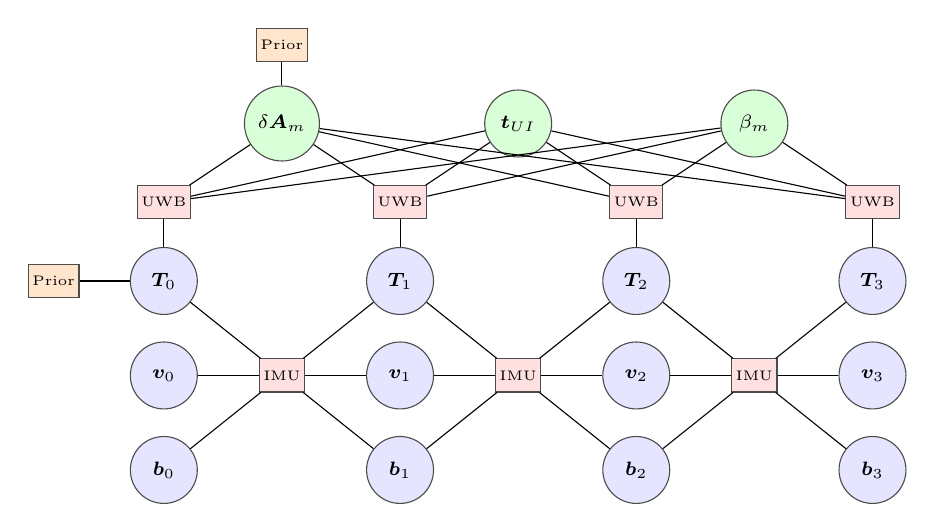
\begin{tikzpicture}[
  var/.style={circle,draw=black!70,fill=blue!10,minimum size=0.85cm,font=\scriptsize},
  fac/.style={rectangle,draw=black!70,fill=red!12,minimum size=0.42cm,font=\tiny,inner sep=1.5pt},
  cal/.style={circle,draw=black!70,fill=green!15,minimum size=0.85cm,font=\scriptsize},
  every node/.style={transform shape}]

% keyframes
\foreach \i/\x in {0/0, 1/3, 2/6, 3/9} {
  \node[var] (X\i) at (\x,0) {$\bT_{\i}$};
  \node[var] (V\i) at (\x,-1.2) {$\bv_{\i}$};
  \node[var] (B\i) at (\x,-2.4) {$\bb_{\i}$};
}
% imu factors
\foreach \i/\j in {0/1,1/2,2/3} {
  \node[fac] (I\i) at ({(\i)*3+1.5},-1.2) {IMU};
  \draw (X\i)--(I\i); \draw (V\i)--(I\i); \draw (B\i)--(I\i);
  \draw (I\i)--(X\j); \draw (I\i)--(V\j); \draw (I\i)--(B\j);
}
% calibration vars
\node[cal] (L) at (4.5,2.0) {$\bt_{UI}$};
\node[cal] (A) at (1.5,2.0) {$\delta\bA_m$};
\node[cal] (Z) at (7.5,2.0) {$\beta_m$};
% uwb factors (one per keyframe to anchor)
\foreach \i/\x in {0/0,1/3,2/6,3/9} {
  \node[fac] (U\i) at (\x,1.0) {UWB};
  \draw (X\i)--(U\i);
  \draw (U\i)--(L); \draw (U\i)--(A); \draw (U\i)--(Z);
}
% priors
\node[fac,fill=orange!20] (P) at (-1.4,0) {Prior};
\draw (P)--(X0);
\node[fac,fill=orange!20] (PA) at (1.5,3.0) {Prior};
\draw (PA)--(A);
\end{tikzpicture}
\caption{因子图示意:关键帧状态(蓝)、标定变量(绿)、因子(红/橙)。每个 UWB 因子同时连接位姿与标定变量。}
\label{fig:fg}
\end{figure}

% #####################################################################
\part{开发 Handbook (Development Handbook)}
% #####################################################################

\chapter{依赖库与开发环境}

\section{核心依赖}
\begin{longtable}{l l p{6cm}}
\toprule
库 & 版本 & 用途 \\
\midrule
GTSAM & $\geq 4.2$ & 因子图优化(含 GNC、CombinedImuFactor、Expression) \\
Eigen3 & $\geq 3.3$ & 线性代数(GTSAM 依赖) \\
Boost & $\geq 1.65$ & GTSAM 依赖 \\
yaml-cpp & $\geq 0.6$ & 配置文件解析 \\
GoogleTest & $\geq 1.11$ & 单元测试 \\
spdlog (可选) & 任意 & 日志 \\
CMake & $\geq 3.16$ & 构建 \\
\bottomrule
\end{longtable}
说明:数据读取可脱离 ROS(直接解析 bag 导出的 csv/二进制),或保留 ROS1/ROS2 适配层。建议\textbf{核心算法不依赖 ROS},以便单测与跨平台。

\section{构建结构}
\begin{lstlisting}[style=cpp]
uwb_imu_fgo/
  CMakeLists.txt
  include/uifgo/        # 公开头文件
  src/                  # 实现
  test/                 # GoogleTest 单元测试
  config/               # yaml 配置
  data/                 # 样例数据
  tools/                # 离线运行入口 (main)
\end{lstlisting}

% ---------------------------------------------------------------------
\chapter{模块划分与依赖}
\begin{figure}[ht]
\centering
\begin{tikzpicture}[node distance=0.55cm and 0.9cm,
  mod/.style={rectangle,rounded corners,draw=black!70,fill=blue!8,
    text width=3.0cm,align=center,minimum height=0.85cm,font=\scriptsize}]
\node[mod] (cfg) {ConfigLoader};
\node[mod,right=of cfg] (data) {DataLoader};
\node[mod,right=of data] (filt) {OutlierFilter\\(NLOS/量程)};
\node[mod,below=of cfg] (init) {Initializer};
\node[mod,below=of data] (imu) {ImuPreintegrator};
\node[mod,below=of filt] (uwb) {UwbRangeFactor};
\node[mod,below=of init] (build) {GraphBuilder};
\node[mod,below=of imu] (opt) {Optimizer\\(GNC+LM)};
\node[mod,below=of uwb] (out) {TrajectoryIO\\\&Evaluator};
\draw[arrow] (cfg)--(init); \draw[arrow] (data)--(filt);
\draw[arrow] (filt)--(uwb); \draw[arrow] (cfg)--(data);
\draw[arrow] (data)--(imu); \draw[arrow] (init)--(build);
\draw[arrow] (imu)--(build); \draw[arrow] (uwb)--(build);
\draw[arrow] (build)--(opt); \draw[arrow] (opt)--(out);
\draw[arrow] (data)--(init);
\end{tikzpicture}
\caption{模块依赖关系}
\label{fig:modules}
\end{figure}

\section{模块职责}
\begin{longtable}{l p{9.5cm}}
\toprule
模块 & 职责 \\
\midrule
\texttt{ConfigLoader} & 解析 yaml:锚点、外参、噪声、求解器参数、阈值 \\
\texttt{DataLoader} & 读取并解析 IMU 与 UWB(\texttt{LinktrackNodeframe3}),单位换算,时间排序 \\
\texttt{OutlierFilter} & RSSI NLOS、量程门限、两步距离一致性前置过滤 \\
\texttt{Initializer} & 静止检测、重力/陀螺偏置、三角定位、yaw 对齐 \\
\texttt{ImuPreintegrator} & 封装 \texttt{PreintegratedCombinedMeasurements},管理帧间积分 \\
\texttt{UwbRangeFactor} & 自定义因子(Expression),含杆臂/锚点/偏置 \\
\texttt{GraphBuilder} & 关键帧化、组装 \texttt{NonlinearFactorGraph} 与初值 \texttt{Values} \\
\texttt{Optimizer} & GNC + 多趟 LM,卡方监控,自标定调度 \\
\texttt{TrajectoryIO} & 轨迹/标定/协方差输出,可选 APE/RPE 评估 \\
\bottomrule
\end{longtable}

% ---------------------------------------------------------------------
\chapter{接口定义}

\section{公共数据类型}
\begin{lstlisting}[style=cpp]
// include/uifgo/types.h
#pragma once
#include <gtsam/geometry/Pose3.h>
#include <Eigen/Core>
#include <vector>
#include <unordered_map>

namespace uifgo {
using gtsam::Vector3; using gtsam::Pose3;

struct ImuSample {
  double t;            // 秒
  Vector3 acc;         // m/s^2 (body)
  Vector3 gyro;        // rad/s (body)
};

struct UwbRange {
  int    anchor_id;
  double dist;         // m
  double fp_rssi;      // dB
  double rx_rssi;      // dB
};

struct UwbFrame {
  double t;            // 秒
  int    tag_id;
  std::vector<UwbRange> ranges;
};

struct AnchorConfig {
  int id;
  Vector3 pos;         // 标称世界系坐标
  double  prior_sigma; // 锚点位置先验 sigma (m)
};

struct NavState {      // 单关键帧结果
  double t;
  Pose3   T;           // body->world
  Vector3 v;
  Vector3 ba, bg;
};
}  // namespace uifgo
\end{lstlisting}

\section{ConfigLoader}
\begin{lstlisting}[style=cpp]
// include/uifgo/config.h
struct Config {
  // 锚点
  std::vector<AnchorConfig> anchors;
  // 外参 & 标定开关
  Vector3 lever_arm_init;     bool calib_lever  = true;
  double  lever_prior_sigma = 0.05;
  bool    calib_anchor = true;
  bool    calib_range_bias = true; double range_bias_sigma = 0.05;
  bool    calib_td = false;   double td_init = 0.03;
  // IMU 噪声
  double sigma_a=0.1, sigma_g=0.01, sigma_wa=0.01, sigma_wg=2e-5;
  double gravity = 9.81;
  // UWB 噪声
  double sigma_range = 0.10;  double v_max = 3.0;
  // 过滤阈值
  double nlos_rssi_diff = 6.0;
  double min_range = 0.3, max_range = 100.0;
  double dist_consistency_thresh = 1.0;
  int    warmup_frames = 20;
  // GNC / 求解器
  int    lm_max_iter = 100; double gnc_inlier_thresh = 1.0;
  // ...
};
class ConfigLoader {
 public:
  static Config Load(const std::string& yaml_path);
};
\end{lstlisting}

\section{DataLoader}
\begin{lstlisting}[style=cpp]
// include/uifgo/data_loader.h
class DataLoader {
 public:
  // 从文件加载;返回按时间升序的序列
  bool LoadImu(const std::string& path, std::vector<ImuSample>* out);
  bool LoadUwb(const std::string& path, std::vector<UwbFrame>* out);
  // 校验: 时间单调、单位、字段完整
};
\end{lstlisting}

\section{OutlierFilter}
\begin{lstlisting}[style=cpp]
// include/uifgo/outlier_filter.h
class OutlierFilter {
 public:
  explicit OutlierFilter(const Config& cfg);
  // 前置硬过滤: 返回保留的 ranges (NLOS/量程)
  std::vector<UwbRange> PreFilter(const UwbFrame& f) const;
  // 距离一致性 (需当前估计位置 + warmup 状态)
  bool ConsistencyOk(const UwbRange& r, const Vector3& p_pred,
                     const Vector3& anchor_pos, bool warmed_up) const;
};
\end{lstlisting}

\section{Initializer}
\begin{lstlisting}[style=cpp]
// include/uifgo/initializer.h
struct InitResult {
  bool ok;
  Pose3 T0; Vector3 v0, ba0, bg0;
  Vector3 gravity_world;   // (0,0,-g) 对齐后
};
class Initializer {
 public:
  Initializer(const Config& cfg);
  // 静止检测 + 重力/陀螺偏置
  bool DetectStatic(const std::vector<ImuSample>&, size_t i0, size_t i1);
  // UWB 三角定位
  bool Trilaterate(const std::vector<UwbRange>&,
                   const std::vector<AnchorConfig>&, Vector3* p_out);
  // 综合初始化
  InitResult Run(const std::vector<ImuSample>&,
                 const std::vector<UwbFrame>&);
};
\end{lstlisting}

\section{ImuPreintegrator}
\begin{lstlisting}[style=cpp]
// include/uifgo/imu_preint.h
#include <gtsam/navigation/CombinedImuFactor.h>
class ImuPreintegrator {
 public:
  ImuPreintegrator(const Config& cfg, const Vector3& gravity_world);
  void Reset(const gtsam::imuBias::ConstantBias& bias);
  void Integrate(const ImuSample& s, double dt);
  // 取出当前累积量以构造 CombinedImuFactor
  const gtsam::PreintegratedCombinedMeasurements& Pim() const;
 private:
  boost::shared_ptr<gtsam::PreintegratedCombinedMeasurements::Params> params_;
  gtsam::PreintegratedCombinedMeasurements pim_;
};
\end{lstlisting}

\section{UwbRangeFactor}
\begin{lstlisting}[style=cpp]
// include/uifgo/uwb_factor.h
#include <gtsam/nonlinear/ExpressionFactor.h>
#include <gtsam/slam/expressions.h>

// 用 Expression 构造残差: r = ||(A+dA)-(R*t_UI+p)|| + beta - z
// 提供工厂函数, 返回可加入图的 ExpressionFactor
namespace uifgo {
gtsam::NonlinearFactor::shared_ptr MakeUwbFactor(
    gtsam::Key pose_key, gtsam::Key lever_key,
    gtsam::Key anchor_key, gtsam::Key bias_key,
    const Vector3& anchor_nominal,
    double measured_range, double sigma,
    bool calib_lever, bool calib_anchor, bool calib_bias);
}
\end{lstlisting}

\section{GraphBuilder}
\begin{lstlisting}[style=cpp]
// include/uifgo/graph_builder.h
#include <gtsam/nonlinear/NonlinearFactorGraph.h>
#include <gtsam/nonlinear/Values.h>
class GraphBuilder {
 public:
  GraphBuilder(const Config& cfg);
  // 输入: 同步后的关键帧数据(UWB帧 + 帧间预积分),输出图与初值
  void Build(const std::vector<UwbFrame>& uwb_kf,
             const std::vector<gtsam::PreintegratedCombinedMeasurements>& pims,
             const InitResult& init,
             gtsam::NonlinearFactorGraph* graph,
             gtsam::Values* values,
             std::vector<size_t>* uwb_factor_indices);
};
\end{lstlisting}

\section{Optimizer}
\begin{lstlisting}[style=cpp]
// include/uifgo/optimizer.h
#include <gtsam/nonlinear/GncOptimizer.h>
struct OptimizeResult {
  gtsam::Values values;
  std::vector<bool> uwb_inlier;   // 与 uwb_factor_indices 对应
  double final_error;
  // 协方差 (可选, 用 Marginals)
};
class Optimizer {
 public:
  Optimizer(const Config& cfg);
  OptimizeResult RunGnc(const gtsam::NonlinearFactorGraph& graph,
                        const gtsam::Values& init,
                        const std::vector<size_t>& uwb_indices);
  OptimizeResult RefineInliers(/* 剔除外点后 LM */ ...);
};
\end{lstlisting}

\section{TrajectoryIO \& Evaluator}
\begin{lstlisting}[style=cpp]
// include/uifgo/trajectory_io.h
class TrajectoryIO {
 public:
  static void WriteTum(const std::string& path,
                       const std::vector<NavState>& traj);
  static void WriteCalib(const std::string& path, const gtsam::Values&);
};
class Evaluator {  // 可选: 有真值时
 public:
  static double AbsoluteTrajectoryError(const std::vector<NavState>&,
                                        const std::vector<NavState>& gt);
};
\end{lstlisting}

% =====================================================================
%  以下两章插入到 Part 2 (开发 Handbook):
%  位置: 第 11 章「接口定义」之后, 第 12 章「开发步骤(里程碑)」之前。
%  依赖主文档导言区已定义的: ctex / listings(style=cpp) /
%  数学宏 \bT \bp \bR \bv \bb \skewop / tikz(decorations.pathreplacing)
% =====================================================================

% #####################################################################
\chapter{UWB Expression 因子参考实现(对应 M4)}
% #####################################################################

本章给出全图中\textbf{唯一需要手写}的因子 \texttt{UwbRangeFactor} 的完整可编译实现。其余因子(IMU、先验)均用 GTSAM 原生类型。核心思路是用 \texttt{gtsam::Expression} 把残差表达式搭出来,由 GTSAM 的自动微分(AD)生成全部雅可比,从而\textbf{不必手推} 4 个变量的解析导数;手推的解析式(设计文档 \S 4.3)仅用于单元测试对拍。

\section{变量类型微调}
设计文档中锚点偏置键 \texttt{Z(m)} 原计划用 \texttt{Vector1} 包裹。为简化 Expression 与先验的书写,这里\textbf{改用原生 \texttt{double}}:GTSAM 对 \texttt{double} 已定义流形 traits(维度 1),可直接用作变量、用 \texttt{Expression<double>} 取叶子、用 \texttt{graph.addPrior<double>} 加先验。其余键不变。

\section{Expression 组合原理}
残差表达式(设计文档 \S 4.3):
\begin{equation}
r_{j,m} = \underbrace{\big\|\,(\bA_m+\delta\bA_m)-(\bR_j\bm{t}_{UI}+\bp_j)\,\big\|}_{\rho_{j,m}} + \beta_m - z_{j,m}.
\end{equation}
按下列三步搭建表达式树:
\begin{enumerate}[leftmargin=2em]
  \item \textbf{天线世界坐标} $\bp_U^W=\bR_j\bm{t}_{UI}+\bp_j$ 用 GTSAM 内置 \texttt{transformFrom(Pose3\_, Point3\_)},它自动提供对位姿(6 dof)与杆臂(3 dof)的雅可比。
  \item \textbf{预测距离} $\rho_{j,m}$ 用\textbf{函数封装表达式}(function-wrapped Expression):把"减去锚点 + 取模"合成一个二元(标定锚点时)或一元(固定锚点时)函数,在函数内部一次性填好对 $\bp_U^W$ 与 $\delta\bA_m$ 的 $1\times3$ 雅可比,避免依赖不确定的 \texttt{Point3} 表达式算子。
  \item \textbf{加偏置} $\rho+\beta$ 用 \texttt{Double\_} 的 \texttt{operator+};再交给 \texttt{ExpressionFactor<double>},其残差自动为 $h(x)-z=(\rho+\beta)-z$。
\end{enumerate}

\paragraph{标定开关 $\to$ 常量叶子(关键技巧)}
当某项标定关闭时,把对应叶子从"变量键"换成"常量值"(如 \verb|Point3_(lever_init)| 而非 \verb|Point3_(lever_key)|)。Expression 会\textbf{自动收集叶子中的变量键},常量叶子不产生键,因此 \texttt{ExpressionFactor} 连接的变量集合随标定开关自动变化,\textbf{无需写多份因子}。

\section{头文件}
\begin{lstlisting}[style=cpp]
// include/uifgo/uwb_factor.h
#pragma once
#include <gtsam/geometry/Pose3.h>
#include <gtsam/geometry/Point3.h>
#include <gtsam/nonlinear/NonlinearFactor.h>

namespace uifgo {

// 工厂函数: 构造紧耦合 UWB 测距因子。
// 残差 r = || (A_nominal + dA) - (R*t_UI + p) || + beta - z
//   pose_key   : X(j)  Pose3   (始终为变量)
//   lever_key  : L(0)  Point3  (calib_lever 时为变量, 否则用 lever_init 常量)
//   anchor_key : A(m)  Point3  (calib_anchor 时为变量 dA, 否则锚点为常量)
//   bias_key   : Z(m)  double  (calib_bias 时为变量 beta, 否则不参与)
gtsam::NonlinearFactor::shared_ptr MakeUwbFactor(
    gtsam::Key pose_key, gtsam::Key lever_key,
    gtsam::Key anchor_key, gtsam::Key bias_key,
    const gtsam::Point3& anchor_nominal,   // 锚点标称世界坐标 A_m
    const gtsam::Point3& lever_init,       // 杆臂初值(关闭标定时用作常量)
    double measured_range,                 // 测距 z_{j,m}
    double sigma,                          // 时间自适应 sigma (设计文档 4.4)
    bool calib_lever, bool calib_anchor, bool calib_bias);

}  // namespace uifgo
\end{lstlisting}

\section{实现(.cpp)}
\begin{lstlisting}[style=cpp]
// src/uwb_factor.cpp
#include "uifgo/uwb_factor.h"
#include <gtsam/nonlinear/ExpressionFactor.h>
#include <gtsam/slam/expressions.h>      // transformFrom(Pose3_, Point3_)
#include <gtsam/nonlinear/expressions.h> // Double_ 算子

namespace uifgo {
using namespace gtsam;

NonlinearFactor::shared_ptr MakeUwbFactor(
    Key pose_key, Key lever_key, Key anchor_key, Key bias_key,
    const Point3& anchor_nominal, const Point3& lever_init,
    double measured_range, double sigma,
    bool calib_lever, bool calib_anchor, bool calib_bias) {

  // ---- 1) 天线世界坐标: p_U^W = R*t_UI + p = transformFrom(T, t_UI)
  Pose3_  pose_(pose_key);
  Point3_ lever_ = calib_lever ? Point3_(lever_key)   // 变量叶子
                               : Point3_(lever_init); // 常量叶子
  Point3_ antenna_ = transformFrom(pose_, lever_);

  // ---- 2) 预测距离 rho = || (A + dA) - p_U^W ||
  //     约定: d = antenna - anchor = p_U - (A+dA), u = d^T/rho
  //     与设计文档 4.3 一致: dr/dp = u^T(经 transformFrom 链式到位姿),
  //                          dr/d(dA) = -u^T
  Double_ dist_;
  if (calib_anchor) {
    auto range_fn = [anchor_nominal](
        const Point3& antenna, const Point3& dA,
        OptionalJacobian<1,3> H_ant,
        OptionalJacobian<1,3> H_dA) -> double {
      Point3   anchor = anchor_nominal + dA;
      Vector3  d = antenna - anchor;
      double   n = d.norm();
      Matrix13 u = (n > 1e-9) ? Matrix13(d.transpose() / n)
                              : Matrix13(Matrix13::Zero()); // 退化保护
      if (H_ant) *H_ant =  u;   // d(rho)/d(antenna)
      if (H_dA)  *H_dA  = -u;   // d(rho)/d(dA)
      return n;
    };
    dist_ = Double_(range_fn, antenna_, Point3_(anchor_key));
  } else {
    auto range_fn = [anchor_nominal](
        const Point3& antenna, OptionalJacobian<1,3> H) -> double {
      Vector3  d = antenna - anchor_nominal;
      double   n = d.norm();
      if (H) *H = (n > 1e-9) ? Matrix13(d.transpose() / n)
                             : Matrix13(Matrix13::Zero());
      return n;
    };
    dist_ = Double_(range_fn, antenna_);
  }

  // ---- 3) 预测测距 = rho + beta (beta 可选)
  Double_ predicted_ = calib_bias ? (dist_ + Double_(bias_key)) : dist_;

  // ---- 4) ExpressionFactor: 残差 = predicted - measured = rho + beta - z
  auto noise = noiseModel::Isotropic::Sigma(1, sigma);
  // 注: GTSAM 4.2 用 boost::shared_ptr; 4.3+ 用 std::shared_ptr,
  //     两者均匹配 NonlinearFactor::shared_ptr。如用 4.3 改为
  //     std::make_shared / gtsam::make_shared。
  return boost::make_shared<ExpressionFactor<double>>(
      noise, measured_range, predicted_);
}

}  // namespace uifgo
\end{lstlisting}

\section{实现要点}
\begin{itemize}[leftmargin=2em]
  \item \textbf{雅可比符号自洽}:函数内 $\bm{u}=\bm{d}^\top/\rho$,$\bm{d}=\bp_U^W-(\bA_m+\delta\bA_m)$。链式经 \texttt{transformFrom} 后 $\partial r/\partial\bp_j=\bm{u}^\top$、$\partial r/\partial\bm{\theta}_j=-\bm{u}^\top\bR_j\skewop{\bm{t}_{UI}}$、$\partial r/\partial\delta\bA_m=-\bm{u}^\top$,与设计文档 \S 4.3 完全一致。$\partial r/\partial\beta_m=1$ 由 \texttt{operator+} 自动给出。
  \item \textbf{零距离退化保护}:$\rho<10^{-9}$ 时雅可比置零,防止除零(物理上 UWB 距离不会为 0,但单测与极端初值可能触发)。
  \item \textbf{时间自适应 $\sigma$}:本因子只接收标量 \texttt{sigma},$\sigma^2=\sigma_{\text{range}}^2+(v_{\max}\Delta t/3)^2$ 在 \texttt{GraphBuilder} 中按帧计算后传入(见下一章)。
  \item \textbf{Expression 自动收集键}:关闭某项标定时对应叶子为常量,因子连接的变量自动减少,无需分支建多种因子。
\end{itemize}

\section{单元测试 UT-6(雅可比数值对拍)}
用 \texttt{numericalDerivative} 校验 AD 雅可比;因子键顺序由 Expression 收集决定,故按键查索引,避免假设顺序。
\begin{lstlisting}[style=cpp]
// test/test_uwb_factor.cpp
#include "uifgo/uwb_factor.h"
#include <gtsam/base/numericalDerivative.h>
#include <gtsam/nonlinear/Values.h>
#include <gtsam/inference/Symbol.h>
#include <gtest/gtest.h>
#include <algorithm>

using namespace gtsam;
using symbol_shorthand::X;  using symbol_shorthand::L;
using symbol_shorthand::A;  using symbol_shorthand::Z;

TEST(UwbFactor, JacobianMatchesNumerical) {
  Point3 anchor(5.0, 4.0, 1.0), lever_init(0.10, 0.0, -0.05);
  Pose3  T(Rot3::RzRyRx(0.1, -0.2, 0.3), Point3(1.0, 2.0, 0.5));
  Point3 dA(0.02, -0.01, 0.03);
  double beta = 0.04, z = 4.0, sigma = 0.1;

  auto f = uifgo::MakeUwbFactor(X(0), L(0), A(0), Z(0),
             anchor, lever_init, z, sigma,
             /*calib_lever=*/true, /*calib_anchor=*/true, /*calib_bias=*/true);

  Values v;
  v.insert(X(0), T); v.insert(L(0), lever_init);
  v.insert(A(0), dA); v.insert<double>(Z(0), beta);

  // 取解析雅可比(unwhitened),并建立 key->H 索引映射
  std::vector<Matrix> H;
  Vector e = f->unwhitenedError(v, H);
  auto Hof = [&](Key k) -> Matrix {
    auto it = std::find(f->keys().begin(), f->keys().end(), k);
    return H[std::distance(f->keys().begin(), it)];
  };

  // 残差值校验: r = ||antenna-anchor*|| + beta - z
  Point3 antenna = T.transformFrom(lever_init);
  double rho = (antenna - (anchor + dA)).norm();
  EXPECT_NEAR(e(0), rho + beta - z, 1e-9);

  // 数值微分逐变量对拍
  auto err_pose = [&](const Pose3& Tp){
    Values vv = v; vv.update(X(0), Tp); return f->unwhitenedError(vv); };
  auto err_lvr  = [&](const Point3& lp){
    Values vv = v; vv.update(L(0), lp); return f->unwhitenedError(vv); };
  auto err_anc  = [&](const Point3& ap){
    Values vv = v; vv.update(A(0), ap); return f->unwhitenedError(vv); };
  auto err_bia  = [&](const double& bp){
    Values vv = v; vv.update(Z(0), bp); return f->unwhitenedError(vv); };

  EXPECT_TRUE(assert_equal(
      numericalDerivative11<Vector,Pose3>(err_pose, T),   Hof(X(0)), 1e-6));
  EXPECT_TRUE(assert_equal(
      numericalDerivative11<Vector,Point3>(err_lvr, lever_init), Hof(L(0)), 1e-6));
  EXPECT_TRUE(assert_equal(
      numericalDerivative11<Vector,Point3>(err_anc, dA),  Hof(A(0)), 1e-6));
  EXPECT_TRUE(assert_equal(
      numericalDerivative11<Vector,double>(err_bia, beta), Hof(Z(0)), 1e-6));
}
\end{lstlisting}
通过判据:残差值误差 $<10^{-9}$,四个变量的 AD 雅可比与数值微分误差 $<10^{-6}$。另需补一个 \texttt{calib\_*} 全关的用例,断言 \verb|f->keys().size()==1|(仅含 \texttt{X(0)})。

% #####################################################################
\chapter{GraphBuilder:关键帧化与 IMU 同步(对应 M5)}
% #####################################################################

本章展开 \texttt{GraphBuilder} 的两件核心工作:\textbf{关键帧化}(在每个 UWB 帧时刻建关键帧)与 \textbf{IMU 时间同步}(把高频 IMU 准确积分到相邻关键帧之间,含边界线性插值)。这是全流程最易出错处:时间对不齐会直接污染 IMU 预积分残差。

\section{关键帧化策略}
\begin{itemize}[leftmargin=2em]
  \item 在\textbf{每个(过滤后)UWB 帧时刻} $t_k$ 建一个关键帧,状态键为 \texttt{X(k),V(k),B(k)}。这样每个 UWB 帧的所有锚点测距都直接约束同一关键帧位姿,无需时间插值即可建 UWB 因子。
  \item UWB 帧率很高时可\textbf{下采样}关键帧(如限制最小间隔 $\Delta t_{\min}$),把被跳过帧的测距合并到最近关键帧或丢弃,以控制问题规模;追求极致精度时保留全部帧。
  \item 跳过\textbf{有效测距数为 0}的帧(过滤后无 range),并保证首帧有足够锚点供初始化三角定位。
\end{itemize}

\section{时间同步与边界插值}
IMU 采样时刻一般与关键帧时刻 $t_k$ 不对齐(图 \ref{fig:timeline})。区间 $[t_{k-1},t_k]$ 的积分采用"\textbf{每个 IMU 样本覆盖其前一段 $\Delta t$}"的约定,并在两端用\textbf{线性插值}得到 $t_{k-1},t_k$ 处的虚拟样本,使积分时长精确等于关键帧间隔。

\begin{figure}[ht]
\centering
\begin{tikzpicture}[font=\small]
\draw[->,thick] (-0.2,0)--(11.2,0) node[right]{$t$};
% IMU 密集采样
\foreach \x in {0.0,0.45,0.9,1.35,1.8,2.25,2.7,3.15,3.6,4.05,4.5,
                4.95,5.4,5.85,6.3,6.75,7.2,7.65,8.1,8.55,9.0,9.45,9.9,10.35,10.8}
  \draw[black!55] (\x,0)--(\x,0.22);
\node[font=\scriptsize,black!55] at (5.4,-0.35) {IMU 高频采样};
% 关键帧
\foreach \x/\lab in {1.1/{$t_{k-1}$}, 5.6/{$t_{k}$}, 9.6/{$t_{k+1}$}} {
  \draw[thick,blue!70] (\x,-0.5)--(\x,0.85);
  \node[blue!70,font=\scriptsize] at (\x,1.05) {\lab};
  \fill[red] (\x,0) circle (1.6pt);
}
\node[red,font=\scriptsize,align=center] at (1.1,-0.85)
  {边界线性插值};
% 积分区间花括号
\draw[decorate,decoration={brace,amplitude=5pt},thick]
  (5.6,1.35)--(1.1,1.35) node[midway,above=4pt,font=\scriptsize]
  {一个 CombinedImuFactor 的预积分区间};
% UWB 因子标注
\node[font=\scriptsize,blue!70,align=center] at (5.6,-0.85)
  {该处建 \texttt{X(k)}\\并加 UWB 因子};
\end{tikzpicture}
\caption{IMU--UWB 时间同步与关键帧化时间线}
\label{fig:timeline}
\end{figure}

\subsection{IMU 预积分器接口微调}
为配合区间积分,\texttt{ImuPreintegrator} 暴露以原始 $(\ba,\bw,\Delta t)$ 为入参的重载:
\begin{lstlisting}[style=cpp]
// include/uifgo/imu_preint.h (在 M3 接口基础上新增重载)
void Reset(const gtsam::imuBias::ConstantBias& bias); // = resetIntegrationAndSetBias
void Integrate(const gtsam::Vector3& acc,
               const gtsam::Vector3& gyro, double dt); // = integrateMeasurement
const gtsam::PreintegratedCombinedMeasurements& Pim() const;
\end{lstlisting}

\subsection{IMU 插值与区间积分(可编译)}
\begin{lstlisting}[style=cpp]
// src/imu_sync.cpp
#include "uifgo/types.h"
#include "uifgo/imu_preint.h"
#include <algorithm>

namespace uifgo {
using gtsam::Vector3;

// 线性插值得到时刻 t 处的 IMU 测量(假设 imu 非空、按时间升序)
ImuSample InterpolateImu(const std::vector<ImuSample>& imu, double t) {
  if (t <= imu.front().t) return imu.front();
  if (t >= imu.back().t)  return imu.back();
  auto it = std::lower_bound(imu.begin(), imu.end(), t,
      [](const ImuSample& s, double v){ return s.t < v; });
  const ImuSample& s1 = *it;
  const ImuSample& s0 = *(it - 1);
  double r = (t - s0.t) / (s1.t - s0.t);
  ImuSample out;
  out.t    = t;
  out.acc  = s0.acc  + r * (s1.acc  - s0.acc);
  out.gyro = s0.gyro + r * (s1.gyro - s0.gyro);
  return out;
}

// 将 [t0, t1] 内的 IMU 积分进 pim;返回新的索引(指向首个 time >= t1 的样本)
// 约定: 每个样本 imu[i] 覆盖区间 (t_prev, imu[i].t]; 两端用插值补齐。
size_t IntegrateBetween(const std::vector<ImuSample>& imu, size_t i,
                        double t0, double t1, ImuPreintegrator* pim) {
  while (i < imu.size() && imu[i].t <= t0) ++i;     // 跳到 t0 之后
  double t_prev = t0;
  while (i < imu.size() && imu[i].t < t1) {         // 中间整段
    double dt = imu[i].t - t_prev;
    if (dt > 1e-9) pim->Integrate(imu[i].acc, imu[i].gyro, dt);
    t_prev = imu[i].t;
    ++i;
  }
  ImuSample s_end = InterpolateImu(imu, t1);        // 末段补到 t1
  double dt = t1 - t_prev;
  if (dt > 1e-9) pim->Integrate(s_end.acc, s_end.gyro, dt);
  return i;
}

}  // namespace uifgo
\end{lstlisting}

\section{GraphBuilder::Build 主流程}
\subsection{算法伪代码}
\begin{lstlisting}[style=cpp]
Build(uwb_kf, imu, init, &graph, &values, &uwb_indices):
  KF  <- [f.t for f in uwb_kf]          # 关键帧时刻(可下采样)
  N   <- len(KF)

  # (1) 首帧先验 + 初值
  graph.addPrior(X(0), init.T0, posePriorNoise)
  graph.addPrior(V(0), init.v0, velPriorNoise)
  graph.addPrior(B(0), bias0,   biasPriorNoise)
  values.insert(X(0)=init.T0, V(0)=init.v0, B(0)=bias0)

  # (2) 标定变量 + 松先验(按开关)
  if calib_lever: values.insert(L(0)=lever_init); graph.addPrior(L(0), lever_init, leverNoise)
  for m in anchors:
    if calib_anchor: values.insert(A(m)=0); graph.addPrior(A(m), 0, anchorNoise[m])
    if calib_bias:   values.insert(Z(m)=0.0); graph.addPrior(Z(m), 0.0, betaNoise)

  # (3) 首帧 UWB 因子
  AddUwbFactorsForFrame(0, uwb_kf[0], graph, uwb_indices)

  # (4) 逐关键帧: IMU 预积分 -> CombinedImuFactor -> 初值传播 -> UWB 因子
  i_imu      <- index of first imu sample > KF[0]
  prev_pose  <- init.T0;  prev_vel <- init.v0;  prev_bias <- bias0
  pim        <- ImuPreintegrator(cfg, gravity_world)
  for k in 1 .. N-1:
    pim.Reset(prev_bias)
    i_imu = IntegrateBetween(imu, i_imu, KF[k-1], KF[k], &pim)
    # CombinedImuFactor 键顺序: pose_i, vel_i, pose_j, vel_j, bias_i, bias_j
    graph.add CombinedImuFactor(X(k-1),V(k-1), X(k),V(k), B(k-1),B(k), pim.Pim())
    pred = pim.Pim().predict(NavState(prev_pose, prev_vel), prev_bias)
    values.insert(X(k)=pred.pose(), V(k)=pred.velocity(), B(k)=prev_bias)
    AddUwbFactorsForFrame(k, uwb_kf[k], graph, uwb_indices)
    prev_pose = pred.pose();  prev_vel = pred.velocity()  # prev_bias 保持初值
\end{lstlisting}

\subsection{C++ 实现}
\begin{lstlisting}[style=cpp]
// src/graph_builder.cpp
#include "uifgo/graph_builder.h"
#include "uifgo/uwb_factor.h"
#include <gtsam/navigation/CombinedImuFactor.h>
#include <gtsam/navigation/NavState.h>
#include <gtsam/slam/PriorFactor.h>
#include <gtsam/inference/Symbol.h>
#include <cmath>

namespace uifgo {
using namespace gtsam;
using symbol_shorthand::X; using symbol_shorthand::V; using symbol_shorthand::B;
using symbol_shorthand::L; using symbol_shorthand::A; using symbol_shorthand::Z;

// 见 src/imu_sync.cpp
size_t IntegrateBetween(const std::vector<ImuSample>&, size_t,
                        double, double, ImuPreintegrator*);

// 时间自适应 sigma: sqrt(sigma_range^2 + (v_max*dt/3)^2)
static double AdaptiveSigma(const Config& c, double dt_since_last) {
  double extra = c.v_max * std::max(0.0, dt_since_last) / 3.0;
  return std::sqrt(c.sigma_range * c.sigma_range + extra * extra);
}

void GraphBuilder::AddUwbFactorsForFrame(
    size_t k, const UwbFrame& f,
    NonlinearFactorGraph* graph, std::vector<size_t>* uwb_indices) {
  for (const UwbRange& r : f.ranges) {
    int m = r.anchor_id;
    const Vector3& A_m  = anchor_pos_.at(m);     // 标称世界坐标
    double dt_anchor    = f.t - last_seen_[m];   // 该锚点距上次测量
    double sigma        = AdaptiveSigma(cfg_, last_seen_.count(m) ? dt_anchor
                                                                  : 0.0);
    auto factor = MakeUwbFactor(X(k), L(0), A(m), Z(m),
                                A_m, cfg_.lever_arm_init,
                                r.dist, sigma,
                                cfg_.calib_lever, cfg_.calib_anchor,
                                cfg_.calib_range_bias);
    size_t idx = graph->size();      // 新因子的索引 = 添加前的图规模
    graph->add(factor);
    uwb_indices->push_back(idx);
    last_seen_[m] = f.t;
  }
}

void GraphBuilder::Build(
    const std::vector<UwbFrame>& uwb_kf,
    const std::vector<ImuSample>& imu,
    const InitResult& init,
    NonlinearFactorGraph* graph, Values* values,
    std::vector<size_t>* uwb_indices) {

  const size_t N = uwb_kf.size();
  const imuBias::ConstantBias bias0(init.ba0, init.bg0);

  // (1) 首帧先验 + 初值
  auto poseN = noiseModel::Diagonal::Sigmas(
      (Vector(6) << 1e-2,1e-2,1e-2, 5e-2,5e-2,5e-2).finished());  // rot, trans
  auto velN  = noiseModel::Isotropic::Sigma(3, 0.1);
  auto biasN = noiseModel::Isotropic::Sigma(6, 1e-2);
  graph->addPrior(X(0), init.T0, poseN);
  graph->addPrior(V(0), init.v0, velN);
  graph->addPrior(B(0), bias0,   biasN);
  values->insert(X(0), init.T0);
  values->insert(V(0), init.v0);
  values->insert(B(0), bias0);

  // (2) 标定变量 + 松先验
  if (cfg_.calib_lever) {
    values->insert(L(0), Point3(cfg_.lever_arm_init));
    graph->addPrior(L(0), Point3(cfg_.lever_arm_init),
                    noiseModel::Isotropic::Sigma(3, cfg_.lever_prior_sigma));
  }
  for (const AnchorConfig& a : cfg_.anchors) {
    anchor_pos_[a.id] = a.pos;
    if (cfg_.calib_anchor) {
      values->insert(A(a.id), Point3(0,0,0));
      graph->addPrior(A(a.id), Point3(0,0,0),
                      noiseModel::Isotropic::Sigma(3, a.prior_sigma));
    }
    if (cfg_.calib_range_bias) {
      values->insert<double>(Z(a.id), 0.0);
      graph->addPrior<double>(Z(a.id), 0.0,
                      noiseModel::Isotropic::Sigma(1, cfg_.range_bias_sigma));
    }
  }

  // (3) 首帧 UWB 因子
  AddUwbFactorsForFrame(0, uwb_kf[0], graph, uwb_indices);

  // (4) 逐关键帧
  ImuPreintegrator pim(cfg_, init.gravity_world);
  size_t i_imu = 0;
  while (i_imu < imu.size() && imu[i_imu].t <= uwb_kf[0].t) ++i_imu;
  Pose3   prev_pose = init.T0;
  Vector3 prev_vel  = init.v0;
  const imuBias::ConstantBias prev_bias = bias0;

  for (size_t k = 1; k < N; ++k) {
    pim.Reset(prev_bias);
    i_imu = IntegrateBetween(imu, i_imu, uwb_kf[k-1].t, uwb_kf[k].t, &pim);

    graph->add(CombinedImuFactor(X(k-1), V(k-1), X(k), V(k),
                                 B(k-1), B(k), pim.Pim()));

    NavState pred = pim.Pim().predict(NavState(prev_pose, prev_vel), prev_bias);
    values->insert(X(k), pred.pose());
    values->insert(V(k), pred.velocity());
    values->insert(B(k), prev_bias);

    AddUwbFactorsForFrame(k, uwb_kf[k], graph, uwb_indices);

    prev_pose = pred.pose();
    prev_vel  = pred.velocity();
  }
}

}  // namespace uifgo
\end{lstlisting}

\section{UWB 因子索引追踪(供 GNC)}
\texttt{uwb\_indices} 记录每个 UWB 因子在图中的下标,供 \texttt{Optimizer} 把\textbf{非 UWB 因子}(IMU、先验)标为 GNC 已知内点:
\begin{lstlisting}[style=cpp]
// Optimizer 内部: 由 uwb_indices 反推 known-inlier 集合
gtsam::GncParams<gtsam::LevenbergMarquardtParams> p;
std::set<size_t> uwb_set(uwb_indices.begin(), uwb_indices.end());
gtsam::GncParams<...>::IndexVector known_inliers;
for (size_t i = 0; i < graph.size(); ++i)
  if (!uwb_set.count(i)) known_inliers.push_back(i);
p.setKnownInliers(known_inliers);  // 只有 UWB 因子参与 GNC 加权
\end{lstlisting}

\section{边界与异常处理}
\begin{itemize}[leftmargin=2em]
  \item \textbf{IMU 数据空洞}:若 $[t_{k-1},t_k]$ 内 IMU 缺失,\texttt{IntegrateBetween} 会退化为单步大 $\Delta t$ 插值,精度下降;应在 \texttt{DataLoader} 校验最大间隔并对超限区间打警告或拆关键帧。
  \item \textbf{首帧无 IMU 前置样本}:\texttt{InterpolateImu} 对越界时刻做端点钳制,保证不越界访问。
  \item \textbf{关键帧间隔为零/逆序}:\texttt{GraphBuilder} 前应断言 \texttt{KF} 严格递增(\texttt{DataLoader} 已排序去重)。
  \item \textbf{帧内重复锚点 ID}:同一帧对同一锚点多次测距应取最优(最小 \texttt{fp\_rssi} 差)或全部加入(独立观测),由 \texttt{OutlierFilter} 决定策略。
\end{itemize}

\section{单元测试 UT-7 与配套用例}
\begin{longtable}{l p{4.4cm} p{6.0cm}}
\toprule
ID & 模块 & 内容与通过判据 \\
\midrule
UT-5b & InterpolateImu & 已知线性段:插值值与解析值误差 $<10^{-12}$;端点钳制正确 \\
UT-5c & IntegrateBetween & 合成匀加速 IMU,区间端点不对齐;\texttt{pim.predict} 与解析位姿误差 $<10^{-6}$,且返回索引正确 \\
UT-7 & GraphBuilder + LM & 无噪声合成轨迹(已知 $\bT_k$ 生成 IMU 与多锚点测距):batch 后 ATE $<10^{-4}$ m;\texttt{uwb\_indices} 数量 = 总测距数 \\
UT-7b & 标定开关 & 关闭全部标定时,图中不含 \texttt{L/A/Z} 变量;各 UWB 因子键数为 1 \\
\bottomrule
\end{longtable}

\paragraph{UT-5c 关键骨架}
\begin{lstlisting}[style=cpp]
// 合成: 真值匀加速运动 + 已知重力, 生成 200Hz IMU,
// 取两个不对齐的关键帧时刻 t0, t1。
ImuPreintegrator pim(cfg, g_world);
pim.Reset(imuBias::ConstantBias());          // 零偏置
IntegrateBetween(imu, 0, t0, t1, &pim);
NavState pred = pim.Pim().predict(NavState(pose0, vel0), imuBias::ConstantBias());
EXPECT_TRUE(assert_equal(pose_gt_t1, pred.pose(), 1e-6));
EXPECT_TRUE(assert_equal(vel_gt_t1,  pred.velocity(), 1e-6));
\end{lstlisting}


% =====================================================================
%  本章插入到 Part 2 (开发 Handbook):
%  位置: 第 13 章「GraphBuilder」之后, 「开发步骤(里程碑)」总表之前。
%  依赖主文档导言区: ctex / listings(style=cpp) /
%  数学宏 \bT \bp \bR \bv \bb / tikz(arrows.meta, positioning)
% =====================================================================

% #####################################################################
\chapter{Optimizer:GNC 鲁棒优化、卡方监控与协方差(对应 M6/M7)}
% #####################################################################

本章实现后端 \texttt{Optimizer}。输入是上一章 \texttt{GraphBuilder} 产出的三件套:因子图 \texttt{graph}、初值 \texttt{values}、UWB 因子下标表 \texttt{uwb\_indices}。核心难点是 UWB 在 NLOS 下会产生\textbf{正偏置粗差}(distance 偏大),必须在保留所有可信约束(IMU、先验)的前提下,只对 UWB 因子做鲁棒处理。我们采用\textbf{三阶段流水线}:GNC 软加权定位粗差 $\to$ 卡方检验硬剔除回环 $\to$ clean 内点图精修并取 \texttt{Marginals}。

\section{理论基础}

\subsection{GNC 鲁棒代价与 known-inliers}
原始最小二乘 $\min_x \tfrac12\sum_i \|e_i(x)\|^2_{\Sigma_i}$ 对粗差敏感。鲁棒 M 估计将其改写为 $\min_x \sum_i \rho\!\big(\|e_i(x)\|_{\Sigma_i}\big)$,其中 $\rho(\cdot)$ 为截断最小二乘(TLS)核。Graduated Non-Convexity(GNC)引入控制参数 $\mu$,把代价从凸($\mu\!\to\!\infty$,近似全内点)逐步同伦到真实非凸 TLS,边优化边求解每个因子的权重 $w_i\in[0,1]$:
\begin{equation}
\hat{x},\,\hat{w} = \arg\min_{x,\,w\in[0,1]^M}\;
\sum_i w_i\,\|e_i(x)\|^2_{\Sigma_i} + \Phi_\mu(w_i),
\end{equation}
收敛时内点 $w_i\!\to\!1$、外点 $w_i\!\to\!0$。\textbf{关键:setKnownInliers} 把 IMU 预积分因子与所有先验因子的权重\textbf{钉死为 1},GNC 的鲁棒"预算"全部用于甄别 UWB 粗差,既防止误删可信的惯性约束,又显著提升收敛稳定性。内点判定阈值 $\bar{c}^2$ 由卡方分位数自动给出:对 $d$ 维因子,$\bar{c}^2 = \tfrac12\,\chi^2_{1-\alpha}(d)$(GTSAM 代价含 $\tfrac12$ 因子)。

\subsection{卡方监控}
GTSAM 的 \texttt{factor->error(x)} 返回 $\tfrac12\|e_i\|^2_{\Sigma_i}$,故白化残差平方为
\begin{equation}
\chi^2_i \;=\; 2\,\texttt{error}_i \;=\; \|e_i(x)\|^2_{\Sigma_i}.
\end{equation}
在零假设(测量正确、噪声高斯)下,$\chi^2_i\sim\chi^2(d_i)$。逐 UWB 因子检验:$\chi^2_i > \chi^2_{1-\alpha}(d_i)$ 则判为外点(UWB 因子 $d_i=1$)。全局拟合优度用\textbf{约化卡方}:
\begin{equation}
\chi^2_\nu = \frac{2\,E(\hat{x})}{\nu},\qquad
\nu = \sum_i d_i - \dim(x),
\end{equation}
其中 $E$ 为全图误差。$\chi^2_\nu\!\approx\!1$ 表示噪声模型与数据相符;$\gg 1$ 表示 $\sigma$ 设小或存在未建模误差;$\ll 1$ 表示 $\sigma$ 设大(过保守)。

\subsection{为何需要 clean 精修(M7 前置)}
GNC 收敛后的图带有鲁棒权重 $w_i$,其线性化信息矩阵 $\sum_i w_i J_i^\top\Sigma_i^{-1}J_i$ \textbf{被人为压低},直接对其取 \texttt{Marginals} 会得到失真(偏乐观或不一致)的协方差。因此 M7 要求:\textbf{在剔除外点后的纯内点图上,用无鲁棒核的标准 LM 再精修一次},该图的信息矩阵才具统计意义,据此求 \texttt{Marginals} 才能给出可上报的位姿/标定不确定度。

\section{三阶段流水线}
\begin{figure}[ht]
\centering
\begin{tikzpicture}[
  node distance=6mm and 9mm, font=\small,
  box/.style={draw,rounded corners,align=center,inner sep=4pt,
              minimum height=8mm, fill=blue!4},
  io/.style={draw,align=center,inner sep=4pt,fill=black!4},
  >=Stealth]
\node[io]  (in)  {graph / values\\uwb\_indices};
\node[box, right=of in]  (gnc) {\textbf{Stage A}\\GNC + TLS\\setKnownInliers\\$\Rightarrow$ 权重 $w_i$};
\node[box, right=of gnc] (rej) {\textbf{Stage B}\\卡方剔除回环\\(clean LM + $\chi^2$ 检验)};
\node[box, right=of rej] (cov) {\textbf{Stage C}\\Marginals\\$\Rightarrow$ 位姿/标定协方差};
\node[io,  right=of cov] (out) {OptimizerResult};
\draw[->] (in)--(gnc);
\draw[->] (gnc)--(rej);
\draw[->] (rej)--(cov);
\draw[->] (cov)--(out);
\draw[->] (rej.south) .. controls +(0,-0.9) and +(0,-0.9) ..
          node[below,font=\scriptsize]{有新外点则回环} (rej.south west);
\end{tikzpicture}
\caption{Optimizer 三阶段流水线}
\label{fig:optpipe}
\end{figure}

\section{Config 扩展字段}
\begin{lstlisting}[style=cpp]
// include/uifgo/config.h (在已有 Config 上新增)
// --- LM 基础 ---
int    lm_max_iter        = 100;
double lm_rel_tol         = 1e-6;
double lm_abs_tol         = 1e-8;
// --- GNC ---
double gnc_mu_step        = 1.4;    // mu 同伦步长(GTSAM 默认)
int    gnc_max_iter       = 50;
double gnc_rel_cost_tol   = 1e-5;
double gnc_inlier_prob    = 0.99;   // 内点代价阈值的卡方置信度
double gnc_weight_thresh  = 0.5;    // 由 GNC 权重硬判内/外点的门限
// --- 卡方剔除回环 ---
int    max_rejection_rounds = 3;
double chi2_reject_prob   = 0.99;   // 逐因子卡方剔除的置信度
\end{lstlisting}

\section{头文件}
\begin{lstlisting}[style=cpp]
// include/uifgo/optimizer.h
#pragma once
#include "uifgo/config.h"
#include <gtsam/nonlinear/NonlinearFactorGraph.h>
#include <gtsam/nonlinear/Values.h>
#include <gtsam/nonlinear/Marginals.h>
#include <gtsam/inference/Key.h>
#include <vector>
#include <set>

namespace uifgo {

struct OptimizerResult {
  gtsam::Values        values;                 // 最终(clean 精修后)状态
  std::vector<size_t>  inlier_uwb_indices;     // 最终内点 UWB 因子下标
  std::vector<size_t>  outlier_uwb_indices;    // 被剔除的 UWB 因子下标
  gtsam::Vector        gnc_weights;            // GNC 收敛权重(对齐 graph 因子)
  double               reduced_chi2 = 0.0;     // clean 图的约化卡方
  int                  num_rejection_rounds = 0;
};

class Optimizer {
 public:
  explicit Optimizer(const Config& cfg) : cfg_(cfg) {}

  // 三阶段流水线主入口
  OptimizerResult Optimize(const gtsam::NonlinearFactorGraph& graph,
                           const gtsam::Values& initial,
                           const std::vector<size_t>& uwb_indices);

  // M7 协方差导出: 必须在 Optimize 之后调用(基于 clean 图)
  gtsam::Matrix Covariance(gtsam::Key key) const;     // 任意变量
  gtsam::Matrix PoseCovariance(size_t k) const;       // X(k) 6x6
  gtsam::Matrix LeverCovariance() const;              // L(0) 3x3
  gtsam::Matrix AnchorCovariance(int m) const;        // A(m) 3x3

 private:
  gtsam::NonlinearFactorGraph BuildCleanGraph(
      const gtsam::NonlinearFactorGraph& full,
      const std::set<size_t>& uwb_set,
      const std::set<size_t>& rejected) const;
  std::vector<size_t> ChiSquareReject(
      const gtsam::NonlinearFactorGraph& full,
      const gtsam::Values& values,
      const std::set<size_t>& uwb_set,
      const std::set<size_t>& already_rejected) const;
  double ReducedChi2(const gtsam::NonlinearFactorGraph& g,
                     const gtsam::Values& v) const;

  Config cfg_;
  // 缓存供 Marginals 复用(Optimize 结束后填充)
  gtsam::NonlinearFactorGraph clean_graph_;
  gtsam::Values               result_values_;
  bool                        solved_ = false;
};

}  // namespace uifgo
\end{lstlisting}

\section{卡方分位数工具}
\begin{lstlisting}[style=cpp]
// src/chi2.cpp
#include <cstddef>
#ifdef UIFGO_USE_BOOST_MATH
#include <boost/math/distributions/chi_squared.hpp>
#endif
namespace uifgo {

// 卡方上分位数 x: P(X <= x) = p, X ~ chi2(dof)。
double Chi2inv(double p, std::size_t dof) {
#ifdef UIFGO_USE_BOOST_MATH
  boost::math::chi_squared dist(static_cast<double>(dof));
  return boost::math::quantile(dist, p);
#else
  // 无 boost 时用查表(覆盖常用小自由度 1..6)。
  // 行: dof; 列: p=0.95 / p=0.99。UWB 因子 dof=1。
  static const double t95[7] = {0, 3.8415, 5.9915, 7.8147,
                                   9.4877, 11.0705, 12.5916};
  static const double t99[7] = {0, 6.6349, 9.2103, 11.3449,
                                  13.2767, 15.0863, 16.8119};
  if (dof >= 1 && dof <= 6) return (p >= 0.99) ? t99[dof] : t95[dof];
  // 超表范围: Wilson-Hilferty 近似
  double z = (p >= 0.99) ? 2.3263 : 1.6449;  // 标准正态分位
  double d = static_cast<double>(dof);
  double c = 1.0 - 2.0/(9.0*d) + z*std::sqrt(2.0/(9.0*d));
  return d * c*c*c;
#endif
}

}  // namespace uifgo
\end{lstlisting}

\section{实现(.cpp)}
\begin{lstlisting}[style=cpp]
// src/optimizer.cpp
#include "uifgo/optimizer.h"
#include <gtsam/nonlinear/LevenbergMarquardtOptimizer.h>
#include <gtsam/nonlinear/GncOptimizer.h>   // 含 GncParams (GTSAM >= 4.1)
#include <gtsam/inference/Symbol.h>

namespace uifgo {
using namespace gtsam;
using symbol_shorthand::X; using symbol_shorthand::L;
using symbol_shorthand::A; using symbol_shorthand::Z;

double Chi2inv(double p, std::size_t dof);   // src/chi2.cpp

// ---------- clean 图: 去掉被剔除的 UWB 因子, 保留全部其它因子 ----------
NonlinearFactorGraph Optimizer::BuildCleanGraph(
    const NonlinearFactorGraph& full,
    const std::set<size_t>& uwb_set,
    const std::set<size_t>& rejected) const {
  NonlinearFactorGraph clean;
  for (size_t i = 0; i < full.size(); ++i) {
    if (!full.at(i)) continue;                      // 跳过空因子位
    if (uwb_set.count(i) && rejected.count(i)) continue;  // 剔除外点 UWB
    clean.add(full.at(i));
  }
  return clean;
}

// ---------- 逐 UWB 因子卡方检验, 返回本轮新增外点(full 图下标) ----------
std::vector<size_t> Optimizer::ChiSquareReject(
    const NonlinearFactorGraph& full, const Values& values,
    const std::set<size_t>& uwb_set,
    const std::set<size_t>& already_rejected) const {
  std::vector<size_t> newly;
  for (size_t i = 0; i < full.size(); ++i) {
    if (!uwb_set.count(i) || already_rejected.count(i)) continue;
    auto f = full.at(i);
    if (!f) continue;
    double chi2   = 2.0 * f->error(values);         // ||whitened||^2
    double thresh = Chi2inv(cfg_.chi2_reject_prob, f->dim());  // dim=1
    if (chi2 > thresh) newly.push_back(i);
  }
  return newly;
}

double Optimizer::ReducedChi2(const NonlinearFactorGraph& g,
                              const Values& v) const {
  double chi2 = 2.0 * g.error(v);
  size_t m = 0;
  for (const auto& f : g) if (f) m += f->dim();     // sum factor dims
  size_t n  = v.dim();                               // sum variable dofs
  size_t nu = (m > n) ? (m - n) : 1;
  return chi2 / static_cast<double>(nu);
}

OptimizerResult Optimizer::Optimize(
    const NonlinearFactorGraph& graph, const Values& initial,
    const std::vector<size_t>& uwb_indices) {

  OptimizerResult out;

  // ---- LM 基础参数(GNC 内层 & clean 精修共用) ----
  LevenbergMarquardtParams lm;
  lm.setMaxIterations(cfg_.lm_max_iter);
  lm.setRelativeErrorTol(cfg_.lm_rel_tol);
  lm.setAbsoluteErrorTol(cfg_.lm_abs_tol);
  // lm.setVerbosityLM("SUMMARY");

  // ====================== Stage A: GNC ======================
  std::set<size_t> uwb_set(uwb_indices.begin(), uwb_indices.end());
  GncParams<LevenbergMarquardtParams>::IndexVector known_inliers; // vector<size_t>
  for (size_t i = 0; i < graph.size(); ++i)
    if (!uwb_set.count(i)) known_inliers.push_back(i);  // IMU + 先验 钉为内点

  GncParams<LevenbergMarquardtParams> gncParams(lm);
  gncParams.setLossType(GncLossType::TLS);              // 截断最小二乘
  gncParams.setKnownInliers(known_inliers);             // 关键: 只鲁棒化 UWB
  gncParams.setMuStep(cfg_.gnc_mu_step);
  gncParams.setMaxIterations(cfg_.gnc_max_iter);
  gncParams.setRelativeCostTol(cfg_.gnc_rel_cost_tol);
  // 用卡方分位数自动设置每个因子的内点代价阈值 barc2 = 0.5*chi2inv(alpha, dim)
  gncParams.setInlierCostThresholdsAtProbability(cfg_.gnc_inlier_prob);

  GncOptimizer<LevenbergMarquardtParams> gnc(graph, initial, gncParams);
  Values gnc_result = gnc.optimize();
  out.gnc_weights   = gnc.getWeights();   // size = graph.size(), 内点接近 1

  // ---- 由 GNC 权重做首轮硬判, 初始化外点集合 ----
  std::set<size_t> rejected;
  for (size_t idx : uwb_indices)
    if (out.gnc_weights(idx) < cfg_.gnc_weight_thresh) rejected.insert(idx);

  // ============ Stage B: 卡方剔除回环 + clean 精修 ============
  Values refined = gnc_result;
  int round = 0;
  for (; round < cfg_.max_rejection_rounds; ++round) {
    NonlinearFactorGraph clean = BuildCleanGraph(graph, uwb_set, rejected);
    // 无鲁棒核的纯 LM, 才能得到正确卡方/协方差
    LevenbergMarquardtOptimizer lmopt(clean, refined, lm);
    refined = lmopt.optimize();

    std::vector<size_t> newly =
        ChiSquareReject(graph, refined, uwb_set, rejected);
    if (newly.empty()) { clean_graph_ = clean; break; }   // 收敛: 无新外点
    rejected.insert(newly.begin(), newly.end());
  }
  // 达到最大轮次仍有剔除: 用最后一轮 clean 图再精修一次定稿
  if (round == cfg_.max_rejection_rounds) {
    clean_graph_ = BuildCleanGraph(graph, uwb_set, rejected);
    LevenbergMarquardtOptimizer lmopt(clean_graph_, refined, lm);
    refined = lmopt.optimize();
  }

  // ---- 汇总结果 ----
  out.values             = refined;
  out.reduced_chi2       = ReducedChi2(clean_graph_, refined);
  out.num_rejection_rounds = round;
  out.outlier_uwb_indices.assign(rejected.begin(), rejected.end());
  for (size_t idx : uwb_indices)
    if (!rejected.count(idx)) out.inlier_uwb_indices.push_back(idx);

  // 缓存供 Stage C (Marginals)
  result_values_ = refined;
  solved_        = true;
  return out;
}

// ====================== Stage C: Marginals ======================
Matrix Optimizer::Covariance(Key key) const {
  if (!solved_)
    throw std::runtime_error("Optimizer::Covariance 调用前需先 Optimize");
  // 在 clean(无鲁棒权重)图上求边缘协方差。CHOLESKY 默认;
  // 若系统不可观可改 Marginals::QR 提升数值稳定。
  Marginals marg(clean_graph_, result_values_, Marginals::CHOLESKY);
  return marg.marginalCovariance(key);   // 不可观时抛 IndeterminantLinearSystem
}
Matrix Optimizer::PoseCovariance(size_t k) const { return Covariance(X(k)); }
Matrix Optimizer::LeverCovariance()      const { return Covariance(L(0)); }
Matrix Optimizer::AnchorCovariance(int m)const { return Covariance(A(m)); }

}  // namespace uifgo
\end{lstlisting}

\section{实现要点}
\begin{itemize}[leftmargin=2em]
  \item \textbf{setKnownInliers 的下标语义}:GNC 的权重向量与 known-inliers 列表均以\textbf{因子在原图中的下标}为索引。\texttt{GraphBuilder} 已经保证 \texttt{uwb\_indices} 记录的是添加时刻的 \texttt{graph.size()},二者天然对齐,补集即为 IMU/先验。
  \item \textbf{$\chi^2=2\cdot\texttt{error}$}:GTSAM 的因子 \texttt{error} 含 $\tfrac12$,务必乘 2 才是白化残差平方;漏乘会让阈值整体偏松一倍。
  \item \textbf{GNC 与卡方双保险}:GNC 的 TLS 已能压低粗差,但其软权重不做硬剔除。卡方回环负责把 $w_i$ 介于灰区($\approx0.3\!\sim\!0.7$)、GNC 未彻底拒绝的边缘外点清掉,并在\textbf{无核 clean 图}上复算残差,避免鲁棒权重掩盖真实超限。
  \item \textbf{回环收敛性}:每轮只\textbf{新增}外点、从不复活,集合单调增长,故至多 \texttt{max\_rejection\_rounds} 轮必停;实践中 1$\sim$2 轮即收敛。
  \item \textbf{协方差必须用 clean 图}:Marginals 直接对 GNC 加权图取协方差会偏乐观;本实现固定使用 \texttt{clean\_graph\_}(内点 + 无核 LM 的线性化),统计上才可上报。
  \item \textbf{不可观处理}:若关闭过多约束或某锚点偏置 $\beta_m$ 不可观,\texttt{Marginals} 会抛 \texttt{IndeterminantLinearSystemException};调用侧应 catch 并提示"该标定量在当前轨迹下不可观,需更激励的运动或锁定该量"。
  \item \textbf{GTSAM 版本}:\texttt{GncOptimizer}/\texttt{GncParams} 自 4.1 起提供;\texttt{setInlierCostThresholdsAtProbability} 在 4.1.1+ 可用,旧版可改用 \texttt{setInlierCostThreshold(0.5*Chi2inv(0.99,1))}(全 UWB 因子同为 1 维,单值阈值即可)。
\end{itemize}

\section{诊断:约化卡方解读}
\begin{longtable}{l p{4.0cm} p{6.2cm}}
\toprule
$\chi^2_\nu$ 区间 & 含义 & 处置 \\
\midrule
$\approx 1$ ($0.8\!\sim\!1.2$) & 噪声模型与数据一致 & 正常,直接采纳协方差 \\
$\gg 1$ & $\sigma$ 设小 / 未建模误差 / 残留外点 & 检查 $\sigma_{\text{range}}$、时间自适应项、收紧卡方剔除 \\
$\ll 1$ ($<0.5$) & $\sigma$ 设大(过保守) & 协方差偏大,可适当调小 $\sigma$ 重跑 \\
\bottomrule
\end{longtable}

\section{单元测试 UT-8 与 UT-9}
\begin{longtable}{l p{3.9cm} p{6.3cm}}
\toprule
ID & 模块 & 内容与通过判据 \\
\midrule
UT-8  & GNC 粗差甄别 & 合成轨迹,对 20\% UWB 测距注入 $+0.8$\,m NLOS 偏置;\texttt{outlier\_uwb\_indices} 与注入集合的 precision/recall 均 $=1$,ATE $<0.05$\,m \\
UT-8b & setKnownInliers & 断言 \texttt{gnc\_weights} 中所有非 UWB 因子下标权重 $=1$;无 IMU/先验被误判 \\
UT-8c & 卡方回环 & 构造一个 GNC 灰区外点($w\!\approx\!0.6$),验证其被卡方轮次剔除,\texttt{num\_rejection\_rounds}$\ge 1$ \\
UT-9  & Marginals & 良条件合成下 \texttt{PoseCovariance} 对称正定,$3\sigma$ 椭球包含真值;不可观用例触发并捕获 \texttt{IndeterminantLinearSystem} \\
UT-9b & 约化卡方 & 正确 $\sigma$ 的高斯噪声合成:多次蒙特卡洛均值 \texttt{reduced\_chi2} $\in[0.9,1.1]$ \\
\bottomrule
\end{longtable}

\paragraph{UT-8 关键骨架}
\begin{lstlisting}[style=cpp]
// 由 GraphBuilder 在合成数据上建图, 对部分 range 注入 NLOS 偏置后建因子。
// injected: 注入偏置的 UWB 因子下标集合(测试侧已知)
uifgo::Optimizer opt(cfg);
auto res = opt.Optimize(graph, values, uwb_indices);

std::set<size_t> got(res.outlier_uwb_indices.begin(),
                     res.outlier_uwb_indices.end());
EXPECT_EQ(got, injected);                         // precision=recall=1

// known-inliers 权重恒为 1
std::set<size_t> uwb_set(uwb_indices.begin(), uwb_indices.end());
for (size_t i = 0; i < graph.size(); ++i)
  if (!uwb_set.count(i)) EXPECT_NEAR(res.gnc_weights(i), 1.0, 1e-9);

// 轨迹精度
EXPECT_LT(ComputeATE(res.values, gt_poses), 0.05);

// 协方差可取且正定
Eigen::Matrix<double,6,6> P = opt.PoseCovariance(K/2);
Eigen::LLT<Eigen::MatrixXd> llt(P);
EXPECT_EQ(llt.info(), Eigen::Success);            // 正定
\end{lstlisting}

% ---------------------------------------------------------------------
\chapter{开发步骤(里程碑)}

每个里程碑都\textbf{可独立编译、运行、用单测验证}后再进入下一步。Codex 应严格按序实现。

\section*{M0 — 脚手架}
\begin{itemize}[leftmargin=2em]
  \item 建立目录、CMake、GoogleTest 接入,空模块编译通过。
  \item \textbf{验证}: \texttt{ctest} 跑空测试成功。
\end{itemize}

\section*{M1 — 数据读取与过滤}
\begin{itemize}[leftmargin=2em]
  \item 实现 \texttt{ConfigLoader}、\texttt{DataLoader}、\texttt{OutlierFilter};其中 \texttt{DataLoader} 解析 \texttt{LinktrackNodeframe3} 的 \texttt{id}、\texttt{dis}、\texttt{fp\_rssi}、\texttt{rx\_rssi} 字段。
  \item \textbf{验证}: UT-1$\sim$UT-3(见 \ref{sec:ut})。能从样例数据输出经过滤的测距序列与时间统计。
\end{itemize}

\section*{M2 — 纯 UWB 三角定位}
\begin{itemize}[leftmargin=2em]
  \item 实现 \texttt{Initializer::Trilaterate},先验证锚点几何与一条粗轨迹(无 IMU)。
  \item \textbf{验证}: UT-4。合成已知位置 + 锚点,恢复误差 $<1$ mm(无噪声),$<\sigma$ 量级(有噪声)。
\end{itemize}

\section*{M3 — IMU 预积分封装}
\begin{itemize}[leftmargin=2em]
  \item 实现 \texttt{ImuPreintegrator},接 GTSAM \texttt{PreintegratedCombinedMeasurements}。
  \item \textbf{验证}: UT-5。匀速/静止/匀加速合成 IMU,预测状态与解析真值一致。
\end{itemize}

\section*{M4 — 自定义 UWB 因子}
\begin{itemize}[leftmargin=2em]
  \item 实现 \texttt{MakeUwbFactor}(Expression)。
  \item \textbf{验证}: UT-6。数值微分校验雅可比与第 4.3 节解析式一致(误差 $<10^{-6}$)。
\end{itemize}

\section*{M5 — 因子图构建 + 紧耦合 batch}
\begin{itemize}[leftmargin=2em]
  \item 实现 \texttt{GraphBuilder} + \texttt{Optimizer}(先用普通 LM,标定关闭),关键帧锚在 UWB 时刻。
  \item \textbf{验证}: UT-7(合成无噪声轨迹应精确恢复),IT-1(样例数据跑通,RMSE 合理)。
\end{itemize}

\section*{M6 — 鲁棒性 GNC + 外点剔除}
\begin{itemize}[leftmargin=2em]
  \item 接入 \texttt{GncOptimizer},打开两步外点剔除。
  \item \textbf{验证}: UT-8(注入 NLOS 外点,GNC 正确标记),IT-2(含 NLOS 数据 RMSE 不退化)。
\end{itemize}

\section*{M7 — 在线自标定}
\begin{itemize}[leftmargin=2em]
  \item 逐项打开:杆臂 $\to$ $\beta_m$ $\to$ $\delta\bA_m$ $\to$ $t_d$。每项打开后看 RMSE 与协方差。
  \item \textbf{验证}: UT-9(注入已知外参/偏置误差,标定后恢复),IT-3(真实数据 RMSE 下降)。
\end{itemize}

\section*{M8 — 多趟精修与输出}
\begin{itemize}[leftmargin=2em]
  \item 实现 multi-pass、卡方监控、TUM 轨迹与标定输出,可选 APE/RPE。
  \item \textbf{验证}: IT-4(端到端,与真值比对 ATE)。
\end{itemize}

% ---------------------------------------------------------------------
\chapter{单元测试规范}\label{sec:ut}

\section{测试原则}
所有数值核都要有\textbf{合成数据(已知真值)}测试 + \textbf{雅可比数值微分对拍}。GTSAM 因子用 \texttt{gtsam::numericalDerivative} 校验。

\section{测试用例清单}
\begin{longtable}{l p{4.2cm} p{6.0cm}}
\toprule
ID & 模块 & 内容与通过判据 \\
\midrule
UT-1 & ConfigLoader & 解析样例 yaml,字段值与期望一致 \\
UT-2 & DataLoader & 解析 \texttt{LinktrackNodeframe3},单位换算、时间单调;畸形输入报错 \\
UT-3 & OutlierFilter & \texttt{rx-fp>6} 被剔除;量程外被剔除;warmup 行为正确 \\
UT-4 & Trilaterate & 合成位置恢复:无噪 $<1$mm;有噪在 $\sigma$ 量级 \\
UT-5 & ImuPreintegrator & 静止/匀速/匀加速:预测位姿误差 $<10^{-6}$ \\
UT-6 & UwbRangeFactor & Expression 雅可比 vs 数值微分 $<10^{-6}$;残差值正确 \\
UT-7 & GraphBuilder+LM & 无噪合成轨迹:ATE $<10^{-4}$ m \\
UT-8 & GNC & 注入 30\% NLOS 外点,inlier 标记 precision/recall $>0.95$ \\
UT-9 & 自标定 & 注入已知杆臂/$\beta_m$/$\delta\bA_m$ 误差,标定后残差 $<$ 先验 \\
UT-10 & 时间自适应协方差 & $\sigma^2$ 随 $\Delta t$ 单调增,公式精确 \\
\bottomrule
\end{longtable}

\section{示例:UWB 因子雅可比测试(UT-6)}
\begin{lstlisting}[style=cpp]
// test/test_uwb_factor.cpp
#include <gtsam/base/numericalDerivative.h>
TEST(UwbFactor, Jacobian) {
  Pose3 T(Rot3::RzRyRx(0.1,-0.2,0.3), Point3(1,2,0.5));
  Point3 lever(0.1,0,0), dA(0,0,0);
  double beta = 0.0, z = /*由真值算*/, sigma = 0.1;
  Vector3 anchor(5,5,1);
  auto factor = uifgo::MakeUwbFactor(X(0),L(0),A(0),B(0),
      anchor, z, sigma, true,true,true);
  Values v; v.insert(X(0),T); v.insert(L(0),lever);
  v.insert(A(0),dA); /* beta via Vector1 */ ...
  // 比较 factor->linearize 与 numericalDerivative
  // 断言 max(|J_auto - J_num|) < 1e-6
}
\end{lstlisting}

% ---------------------------------------------------------------------
\chapter{集成测试与验证}

\begin{longtable}{l p{4cm} p{6.5cm}}
\toprule
ID & 场景 & 通过判据 \\
\midrule
IT-1 & 干净仿真数据(无外点) & ATE RMSE $<$ UWB 测距 $\sigma$ \\
IT-2 & 注入 NLOS 的仿真 & 开 GNC 后 ATE 不退化($<1.2\times$ IT-1) \\
IT-3 & 注入系统误差(锚点/外参偏) & 开自标定后 ATE 显著下降($>30\%$) \\
IT-4 & 真实数据 + 真值(若有) & ATE 报告,人工核对轨迹无发散 \\
IT-5 & 退化轨迹(激励不足) & 标定变量协方差大时自动回退先验,不发散 \\
\bottomrule
\end{longtable}

\section{诊断输出(必须)}
每次运行输出:每因子卡方分布直方图、GNC 内/外点比例、各标定变量后验 $\pm\sigma$、收敛迭代曲线。用于判断是否欠/过标定。

% ---------------------------------------------------------------------
\chapter{配置文件规范}
\begin{lstlisting}[style=yaml]
# config/slam.yaml
anchors:
  - {id: 101, pos: [0.0, 0.0, 0.0], prior_sigma: 0.08}
  - {id: 102, pos: [5.0, 0.0, 0.0], prior_sigma: 0.08}
  - {id: 103, pos: [5.0, 5.0, 2.0], prior_sigma: 0.08}
  - {id: 104, pos: [0.0, 5.0, 2.0], prior_sigma: 0.08}

extrinsics:
  lever_arm_init: [0.0, 0.0, 0.0]   # UWB 天线在 IMU 系
  calib_lever: true
  lever_prior_sigma: 0.05

calibration:
  calib_anchor: true
  calib_range_bias: true
  range_bias_sigma: 0.05
  calib_td: false
  td_init: 0.03

imu:
  sigma_a: 0.1
  sigma_g: 0.01
  sigma_wa: 0.01
  sigma_wg: 2.0e-5
  gravity: 9.81

uwb:
  sigma_range: 0.10
  v_max: 3.0
  nlos_rssi_diff: 6.0
  min_range: 0.3
  max_range: 100.0
  dist_consistency_thresh: 1.0
  warmup_frames: 20

solver:
  lm_max_iter: 100
  rel_error_tol: 1.0e-6
  abs_error_tol: 1.0e-8
  use_gnc: true
  gnc_inlier_thresh: 1.0
\end{lstlisting}

% ---------------------------------------------------------------------
\appendix
\chapter{连续时间升级路径(可选 Plan B)}\label{app:ct}
若后续需要更高精度或加入 LiDAR/相机/高频 TDoA,可将离散关键帧替换为\textbf{累积三次 B 样条控制点}:位置用欧氏 B 样条插值,姿态用 $\log/\exp$ 流形插值(SFUISE 方法);IMU 残差改为对样条求解析导数 $\ddot{\bp},\bw$ 直接比对原始 IMU(免预积分);UWB 残差在精确测量时刻查询样条。GTSAM 无原生 B 样条因子,需自写控制点因子,工程量明显更大,故为 Plan B。本设计的状态接口与因子框架已为该升级预留(关键帧抽象 $\to$ 控制点抽象)。

\chapter{术语与缩写}
\begin{longtable}{l l}
\toprule
缩写 & 全称 \\
\midrule
FGO & Factor Graph Optimization \\
GNC & Graduated Non-Convexity \\
TLS & Truncated Least Squares \\
TWR & Two-Way Ranging \\
TDoA/ToA & Time-(Difference-)of-Arrival \\
NLOS & Non-Line-of-Sight \\
ATE/RPE & Absolute/Relative Pose Error \\
\bottomrule
\end{longtable}

\end{document}